\chapter{Learning Frequencies from Data}\label{ch:sparse-frequency}

\begin{chapterintro}
Strike two tuning forks at once and record the sound. If someone hands you the recording and tells you only that it was made by "a few tuning forks", you can recover their pitches: you look for the strongest periodic component, take it out, look again, and stop when nothing periodic is left. If instead you were told nothing, and you tried to describe the recording with a huge, flexible set of wiggles, you could reproduce the recording perfectly and still have no idea what the next second will sound like.

This chapter is about that difference. In Chapter~\ref{ch:explicit-formula} you learned that the fluctuating part of the zero-counting function of the Riemann zeta function is, approximately, a sum of sinusoids in the height $t$, with angular frequencies $m\log p$ fixed by the primes. Here we ask a learning question: if you did not know that formula, could you discover those frequencies from the zeros alone? We build three kinds of fitted sinusoidal model: one told the frequencies, one given a dense uniform grid of frequencies, and one told only that a \emph{few} frequencies suffice. We derive why the first and third generalize to unseen zeros and the second does not, how precisely a frequency can be learned from a finite window, why skill decays far from that window, how to decide whether a learned frequency "is" the logarithm of a prime power, and why turning a fitted sum of sinusoids back into predicted zeros can be ambiguous.

Where this shows up in the paper: these are the "fitted sinusoidal controls" of Sec.~II~D of the paper \cite{soniR1}, labelled B, C1 and C2, whose results fill Table~IV and the paragraph "Comparable budgets and fitted controls" of Sec.~IV; their recipe is step~(20) of Appendix~A, and the surrogate check of their frequencies is step~(23). They are what lets the paper say that "the obstacle is the parametrization, not the parameter count".
\end{chapterintro}

\begin{prerequisites}

\item Chapter~\ref{ch:fourier-transform}: the Fourier transform of a finite-length sinusoid (a sinc), the resolution $\Delta\omega\approx2\pi/T$ of a window of length $T$, the periodogram, leakage, phase randomization.
\item Chapter~\ref{ch:least-squares}: linear least squares, normal equations, the singular value decomposition (SVD), the condition number, ridge regularization with filter factors $\sigma/(\sigma^2+\lambda\sigma_1^2)$, underdetermined systems and the minimum-norm solution.
\item Chapter~\ref{ch:explicit-formula}: the truncated explicit formula $\Nfl(t)$ (paper Eq.~(4)), predicting zeros by solving $\Nsm(t)+\Nfl(t)=n-\tfrac12$, and Landau's formula that puts peaks at $\log p^m$.
\item Chapter~\ref{ch:generalization}: training and held-out data, the null model, saturated models, interpolation versus extrapolation, inductive bias.
\item Chapter~\ref{ch:controls}: bootstrap intervals, surrogate data, exploratory versus confirmatory analysis.
\item First-year physics: sinusoids, superposition, beats.

\end{prerequisites}

%======================================================================
\section{What it means to learn a frequency}\label{sec:sparse-frequency-why}

\subsection{The data: one number per zero}

Recall the setting. The $n$-th nontrivial zero of the Riemann zeta function is $\rho_n=\tfrac12+\ii t_n$, and $t_n>0$ is its \emph{height}; the first is $t_1=14.134725$ (running example RE1). The counting function $N(t)$ is the number of zeros with $0<t_n\le t$. Recall from Chapter~\ref{ch:counting-zeros} that it splits as
\begin{equation}
N(t)=\Nsm(t)+S(t),\qquad
\Nsm(t)=\frac{t}{2\pi}\log\frac{t}{2\pi}-\frac{t}{2\pi}+\frac78,
\label{eq:sparse-frequency-nsm}
\end{equation}
up to a term of order $1/t$, where $\Nsm$ (paper Eq.~(1)) is the smooth part and $S(t)$ is the small fluctuating part. Throughout, $\log$ is the natural logarithm. The \emph{smooth zeros} $s_n$ solve $\Nsm(s_n)=n-\tfrac12$, and the local mean spacing is $\gap_n=\dd s_n/\dd n$.

At $t=t_n$ the step function $N(t)$ jumps from $n-1$ to $n$. The midpoint of the jump is $n-\tfrac12$, so if we evaluate the decomposition \eqref{eq:sparse-frequency-nsm} at the midpoint of the jump we get $n-\tfrac12=\Nsm(t_n)+S(t_n)$, where $S(t_n)$ means the midpoint value of $S$ at its jump. This motivates the definition of the \textbf{training target}
\begin{equation}
y_n \;=\; n-\tfrac12-\Nsm(t_n)\;\approx\; S(t_n).
\label{eq:sparse-frequency-target}
\end{equation}
Each zero supplies one number $y_n$, attached to one position $t_n$. The positions are irregular: they are the zeros themselves.

How does $y_n$ relate to the fluctuation measured in mean spacings, $(t_n-s_n)/\gap_n$, which is how the paper scores everything? Expand $\Nsm$ about $s_n$ by Taylor's theorem (Chapter~\ref{ch:asymptotics}):
\begin{align}
\Nsm(t_n)&=\Nsm(s_n)+\Nsm'(s_n)(t_n-s_n)+\tfrac12\Nsm''(\xi)(t_n-s_n)^2 \quad\text{(some $\xi$ between $s_n$ and $t_n$)}\notag\\
&=n-\tfrac12+\Nsm'(s_n)(t_n-s_n)+\tfrac12\Nsm''(\xi)(t_n-s_n)^2 .
\end{align}
To find $\Nsm'(s_n)$, treat $n$ as continuous and differentiate the identity $\Nsm(s_n)=n-\tfrac12$ with respect to $n$ using the chain rule:
\begin{equation}
\Nsm'(s_n)\,\frac{\dd s_n}{\dd n}=1
\quad\Longrightarrow\quad
\Nsm'(s_n)=\frac{1}{\gap_n}.
\label{eq:sparse-frequency-slope-gap}
\end{equation}
Substituting and rearranging,
\begin{equation}
y_n=n-\tfrac12-\Nsm(t_n)\approx-\frac{t_n-s_n}{\gap_n}.
\label{eq:sparse-frequency-yfluct}
\end{equation}
The neglected term is $\tfrac12\Nsm''(t_n-s_n)^2$. Differentiating \eqref{eq:sparse-frequency-nsm} twice gives $\Nsm''(t)=1/(2\pi t)$, so for a displacement of one full spacing at zero 400 ($t\approx680$, $\gap\approx1.34$) the neglected term is $1.34^2/(4\pi\cdot680)\approx2\times10^{-4}$, utterly negligible. So: \emph{$y_n$ is minus the fluctuation in mean spacings}, and an error of $0.01$ in $y$ is an error of about $0.01$ mean spacings in the zero.

\subsection{What the explicit formula says the data look like}

Chapter~\ref{ch:explicit-formula} gave the (heuristic, truncated) approximation
\begin{equation}
S(t)\approx \Nfl(t)=-\frac1\pi\sum_{p\in P}\sum_{m=1}^{3}\frac{\sin(mt\log p)}{m\,p^{m/2}},
\label{eq:sparse-frequency-nfl}
\end{equation}
the paper's Eq.~(4), where $P$ is a set of primes $p$. Each term is a sinusoid in $t$ with angular frequency $\omega=m\log p$, that is, $\omega=\log q$ for the prime power $q=p^m$. (Angular frequency "in $t$" means the term repeats when $t$ grows by $2\pi/\omega$; for $p=2$, $m=1$ that period is $2\pi/\log2\approx9.065$, running example RE2.) So the data $y_n$ are samples, at irregular points $t_n$, of a function that is (approximately) a sum of sinusoids with frequencies we know.

The question of this chapter is: \emph{suppose we pretend not to know those frequencies.} How much would a learner have to be told in order to predict zeros it has not seen?

\subsection{Three levels of supplied information}

The paper (Sec.~IV) organizes its models by what they are told. \Cref{tab:sparse-frequency-levels} lists them. The truncated explicit formula, which the paper calls the oracle, is told everything and fits nothing. At the other end, a fitted potential (Chapters~\ref{ch:fitting} and~\ref{ch:generalization}) or a dense grid of frequencies is told nothing structural at all. In between sits a model told only "the answer is a sum of a few sinusoids in $t$".

\begin{table}[htbp]\centering
\caption{The three levels of supplied information in the paper's Sec.~IV, with the model labels of its Sec.~II~D and Table~IV.}
\label{tab:sparse-frequency-levels}
\begin{tabular}{lll}
\toprule
level & what the model is told & models \\
\midrule
(i) & the frequencies $m\log p$ & A (oracle, nothing fitted), B (amplitudes fitted)\\
(ii) & only "few frequencies" (sparsity) & C2 (greedy sparse search)\\
(iii) & nothing structural (generic basis) & C1 (dense uniform grid), fitted potentials\\
\bottomrule
\end{tabular}
\end{table}

All the fitted controls share one shape. A function
\begin{equation}
F(t)=\sum_{j=1}^{J}\bigl[a_j\sin(\omega_j t)+b_j\cos(\omega_j t)\bigr]
\label{eq:sparse-frequency-model}
\end{equation}
is fitted so that $F(t_n)\approx y_n$ on the training zeros, and then the $n$-th zero is predicted by solving the \textbf{level equation}
\begin{equation}
\Nsm(t)+F(t)=n-\tfrac12
\label{eq:sparse-frequency-level}
\end{equation}
for $t$, exactly as the oracle solves $\Nsm+\Nfl=n-\tfrac12$. What differs between B, C1 and C2 is only how the frequencies $\omega_j$ are chosen.

Why is fitting $F(t_n)\approx y_n$ the right thing to do if we care about zeros? Let $\hat t_n$ solve \eqref{eq:sparse-frequency-level}. Subtract the definition $n-\tfrac12=\Nsm(t_n)+y_n$ from \eqref{eq:sparse-frequency-level}:
\begin{equation}
\Nsm(\hat t_n)-\Nsm(t_n)=y_n-F(\hat t_n).
\end{equation}
To first order in $\hat t_n-t_n$, the left side is $(\hat t_n-t_n)/\gap_n$ by \eqref{eq:sparse-frequency-slope-gap}, and $F(\hat t_n)\approx F(t_n)+F'(t_n)(\hat t_n-t_n)$. Collecting the terms in $\hat t_n-t_n$,
\begin{equation}
\frac{\hat t_n-t_n}{\gap_n}\approx\frac{y_n-F(t_n)}{1+F'(t_n)\,\gap_n}.
\label{eq:sparse-frequency-errorlink}
\end{equation}
When $\abs{F'}\gap_n\ll1$, the error of the predicted zero in mean spacings is just the fitting residual $y_n-F(t_n)$. We will meet the condition on $F'$ again in \cref{sec:sparse-frequency-roots}, where it decides whether \eqref{eq:sparse-frequency-level} has one root or several.

\begin{keyideas}
\item The data are one number per zero, $y_n=n-\tfrac12-\Nsm(t_n)\approx S(t_n)$, sampled at the irregular heights $t_n$; to excellent accuracy $y_n$ is minus the fluctuation in mean spacings, \eqref{eq:sparse-frequency-yfluct}.
\item The explicit formula says $y_n$ is approximately a sum of sinusoids with frequencies $\log q$, $q$ a prime power.
\item All fitted controls fit $F(t)$ of form \eqref{eq:sparse-frequency-model} to $y_n$ and predict zeros from $\Nsm(t)+F(t)=n-\tfrac12$; they differ in how much they are told about the frequencies.
\end{keyideas}

%======================================================================
\section{Sinusoidal regression with known frequencies}\label{sec:sparse-frequency-known}

\subsection{Linear in amplitudes, nonlinear in frequency}

Look at \eqref{eq:sparse-frequency-model} with the frequencies $\omega_j$ fixed. Then $F(t)$ depends on the $2J$ numbers $a_j,b_j$ \emph{linearly}: doubling every $a_j$ and $b_j$ doubles $F$. Fitting them to data is therefore linear least squares (Chapter~\ref{ch:least-squares}). Stack the $n_{\rm fit}$ targets into a vector $\bm y$ and the unknowns into
\begin{equation}
\bm c=(a_1,\dots,a_J,\;b_1,\dots,b_J)^\top .
\end{equation}
The \textbf{design matrix} $X$ has one row per training zero and one column per unknown:
\begin{equation}
X_{n,j}=\sin(\omega_j t_n),\qquad X_{n,J+j}=\cos(\omega_j t_n),\qquad n=1,\dots,n_{\rm fit},\; j=1,\dots,J.
\label{eq:sparse-frequency-design}
\end{equation}
Then the vector of model values at the training zeros is $X\bm c$, and least squares minimizes $\norm{\bm y-X\bm c}^2$. Recall from Chapter~\ref{ch:least-squares} that the minimizer satisfies the normal equations
\begin{equation}
X^\top X\,\bm c = X^\top\bm y .
\label{eq:sparse-frequency-normal}
\end{equation}

If instead the frequencies are unknown, $F$ depends on each $\omega_j$ through $\sin(\omega_j t)$, which is not linear in $\omega_j$; frequency estimation is a nonlinear problem. The strategy of this whole chapter is to \emph{choose} frequencies by some rule and then solve the easy linear problem for the amplitudes.

\begin{checkpoint}
Is the model $a\sin(\omega t)+b\cos(\omega t)$ linear in $\omega$? Is it linear in $(a,b)$?
\end{checkpoint}
\checkanswer{Not in $\omega$: replacing $\omega$ by $2\omega$ does not double the function. Yes in $(a,b)$: the function is $a$ times one fixed function plus $b$ times another.}

\subsection{Amplitude and phase}

The pair $a\sin\omega t+b\cos\omega t$ is a single sinusoid in disguise. Write $a=R\cos\varphi$ and $b=R\sin\varphi$ with
\begin{equation}
R=\sqrt{a^2+b^2},\qquad \varphi=\operatorname{atan2}(b,a),
\label{eq:sparse-frequency-ampphase}
\end{equation}
where $\operatorname{atan2}(b,a)$ is the angle of the point $(a,b)$ in the plane, measured from the positive horizontal axis. Then, by the addition formula $\sin(\alpha+\beta)=\sin\alpha\cos\beta+\cos\alpha\sin\beta$,
\begin{equation}
R\sin(\omega t+\varphi)=R\cos\varphi\,\sin\omega t+R\sin\varphi\,\cos\omega t=a\sin\omega t+b\cos\omega t .
\end{equation}
Fitting $(a,b)$ is therefore the same as fitting an amplitude $R$ and a phase $\varphi$, but in a form where the unknowns enter linearly.

\begin{sample}{A four-point fit with a known frequency}
Fit $a\sin t+b\cos t$ (so $\omega=1$) to the data $y=1.1,\;2.0,\;-0.9,\;-2.2$ at $t=0,\;\pi/2,\;\pi,\;3\pi/2$. Find $a$, $b$, the amplitude, the phase and the rms residual.

\textbf{Step 1: design matrix.} Row $n$ is $(\sin t_n,\cos t_n)$: $(0,1)$, $(1,0)$, $(0,-1)$, $(-1,0)$.

\textbf{Step 2: $X^\top X$.} The $(1,1)$ entry is $\sum\sin^2t_n=0+1+0+1=2$; the $(2,2)$ entry is $\sum\cos^2t_n=1+0+1+0=2$; the off-diagonal entry is $\sum\sin t_n\cos t_n=0$, since every row has a zero. So $X^\top X=\mathrm{diag}(2,2)$.

\textbf{Step 3: $X^\top\bm y$.} Sine column: $0(1.1)+1(2.0)+0(-0.9)+(-1)(-2.2)=4.2$. Cosine column: $1(1.1)+0(2.0)+(-1)(-0.9)+0(-2.2)=2.0$.

\textbf{Step 4: solve \eqref{eq:sparse-frequency-normal}.} $a=4.2/2=2.1$, $b=2.0/2=1.0$.

\textbf{Step 5: amplitude and phase.} $R=\sqrt{2.1^2+1.0^2}=\sqrt{5.41}=2.326$, $\varphi=\operatorname{atan2}(1.0,2.1)=0.444$~rad.

\textbf{Step 6: residuals.} The fitted values are $b,\;a,\;-b,\;-a=1.0,\;2.1,\;-1.0,\;-2.1$, so the residuals $y-\hat y$ are $0.1,\,-0.1,\,0.1,\,-0.1$, rms $0.1$.

$$\boxed{a=2.1,\quad b=1.0,\quad R\approx2.326,\quad \varphi\approx0.444\ \text{rad},\quad \text{rms residual}=0.1}$$
\end{sample}

\subsection{When are the columns nearly orthogonal?}

In the sample, $X^\top X$ came out diagonal, so each amplitude was found independently of the other. With many frequencies and many irregular samples this is not exact, but it is nearly true when the frequencies are well separated. Here is why.

A typical entry of $X^\top X$, divided by the number of samples, is an average such as $\frac1n\sum_n\sin(\omega_i t_n)\sin(\omega_j t_n)$. Use $\sin\alpha\sin\beta=\tfrac12[\cos(\alpha-\beta)-\cos(\alpha+\beta)]$:
\begin{equation}
\frac1n\sum_n\sin(\omega_i t_n)\sin(\omega_j t_n)=\frac12\Bigl[\frac1n\sum_n\cos(\delta_-t_n)-\frac1n\sum_n\cos(\delta_+t_n)\Bigr],
\quad \delta_\mp=\omega_i\mp\omega_j .
\end{equation}
\emph{Approximation:} if the samples are spread fairly evenly over a window of length $T$ centred at $t_c$, and many samples fall within each period of the cosines, the average over samples is close to the average over the window. (For the zeros the sample density is not uniform: it grows with height. That changes the weights but not the conclusion below.) The window average is
\begin{align}
\frac1T\int_{t_c-T/2}^{t_c+T/2}\cos(\delta t)\,\dd t
&=\frac{1}{\delta T}\Bigl[\sin\bigl(\delta(t_c+\tfrac T2)\bigr)-\sin\bigl(\delta(t_c-\tfrac T2)\bigr)\Bigr]\notag\\
&=\frac{1}{\delta T}\,2\cos(\delta t_c)\sin\bigl(\tfrac{\delta T}{2}\bigr)\quad\text{($\sin A-\sin B=2\cos\tfrac{A+B}{2}\sin\tfrac{A-B}2$)}\notag\\
&=\cos(\delta t_c)\,\frac{\sin(\delta T/2)}{\delta T/2}.
\label{eq:sparse-frequency-orth}
\end{align}
The factor $\sin(x)/x$ with $x=\delta T/2$ is the sinc function of Chapter~\ref{ch:fourier-transform}: it equals 1 at $x=0$ and is at most $1/\abs{x}=2/(\abs\delta T)$ in magnitude for $x\ne0$. So:
\begin{itemize}
\item For $i=j$, $\delta_-=0$ and the diagonal entry is $\tfrac12[1-(\text{small})]\approx\tfrac12$.
\item For $i\ne j$ with $\abs{\omega_i-\omega_j}\gg2\pi/T$, both terms are small, and the columns are nearly orthogonal.
\item For $\abs{\omega_i-\omega_j}\lesssim2\pi/T$, the first term is close to $\tfrac12\cos(\delta_- t_c)$; the two columns are nearly parallel, $X^\top X$ is nearly singular, and (Chapter~\ref{ch:least-squares}) the condition number is large and noise is amplified.
\end{itemize}
This is the \textbf{resolution limit} of Chapter~\ref{ch:fourier-transform}, now in least-squares language: two frequencies closer than about $2\pi/T$ cannot be told apart by a window of length $T$.

\subsection{Control B: the frequencies $m\log p$ given}

The paper's control B takes the frequencies of the oracle, $\omega=m\log p$ for $m=1,2,3$ and a set of primes, and fits the amplitudes to the training zeros with ridge regularization. Recall the ridge solution from Chapter~\ref{ch:least-squares}: with the SVD $X=U\Sigma V^\top$ and singular values $\sigma_1\ge\sigma_2\ge\dots$,
\begin{equation}
\bm c=V\,\mathrm{diag}\!\left(\frac{\sigma_i}{\sigma_i^2+\lambda\sigma_1^2}\right)U^\top\bm y ,
\label{eq:sparse-frequency-ridge}
\end{equation}
which is exactly the filter of the paper's Appendix~A step~(20). Directions with $\sigma_i^2\gg\lambda\sigma_1^2$ are fitted almost as plain least squares; directions with $\sigma_i^2\ll\lambda\sigma_1^2$ are suppressed.

\begin{sample}{Budgets of the known-frequency controls}
The paper's Table~IV lists control B with 25 primes (150 fitted parameters) and with 150 primes (900 fitted parameters), and the oracle A with 300 primes (900 terms). (a)~Confirm these counts. (b)~Which primes are the 25th, 150th and 300th? (c)~What is the largest frequency in the 25-prime set? (d)~For 900 coefficients and 400 training zeros, is the least-squares problem over- or underdetermined?

\textbf{Step 1: count.} Each prime contributes $m=1,2,3$: three frequencies. Each frequency carries two coefficients $(a,b)$. With 25 primes: $75$ frequencies, $150$ coefficients. With 150 primes: $450$ frequencies, $900$ coefficients. The oracle with 300 primes has $300\times3=900$ terms, none fitted.

\textbf{Step 2: primes.} Listing primes (Chapter~\ref{ch:primes}), the 25th is $97$, the 150th is $863$ and the 300th is $1987$.

\textbf{Step 3: largest frequency.} $3\log97=3(4.5747)=13.724$.

\textbf{Step 4: determinacy.} Unknowns per equation: $900/400=2.25>1$. There are more unknowns than equations, so (Chapter~\ref{ch:least-squares}) there are infinitely many exact fits and the data alone cannot pin down the coefficients.

$$\boxed{150\ \text{and}\ 900\ \text{coefficients};\ p_{25}=97,\ p_{150}=863,\ p_{300}=1987;\ \omega_{\max}=13.72;\ \text{underdetermined (ratio }2.25)}$$
\end{sample}

The paper reports (Sec.~IV and Table~IV) that B with 25 primes gives held-out rms $0.028$ and correlation $+0.99$ on zeros 401--500 from 400 training zeros, \emph{better} than the unfitted 25-prime oracle ($0.043$/$+0.99$). Fitting the amplitudes helps because the truncated formula leaves out everything beyond $p\le97$ and $m\le3$; fitted amplitudes can partly absorb leftover structure at nearby frequencies. With 900 coefficients on 400 zeros, B degrades to $0.180$/$+0.78$, yet it stays below the null $0.263$ and positively correlated. Why does an underdetermined fit still predict something? The paper reports the numbers but does not offer an explanation; what follows is our heuristic reading. Every candidate $F$ in this family, however badly its amplitudes are pinned, is built only from the correct frequencies, so whatever pattern it fits in the window is continued at the right frequencies outside it. This is not a guarantee: large, partly cancelling amplitudes that cancel only inside the window can extrapolate badly, and the degradation of this row from $0.028$ to $0.180$ shows that some such damage does occur. With 800 training zeros the same 900-coefficient model improves to $0.100$/$+0.94$, as more data pin the amplitudes.

\begin{pycode}
import numpy as np, qmnt
def Nsm(t):
    u = np.asarray(t)/(2*np.pi); return u*np.log(u) - u + 7/8
nfit = 400
t = qmnt.zeros(500)
n = np.arange(1, 501)
y = n - 0.5 - Nsm(t)                      # targets y_n, approx S(t_n)
P = qmnt.first_primes(25)
om = np.array([m*np.log(p) for p in P for m in (1, 2, 3)])
def design(tt, om):
    tt = np.atleast_1d(tt)
    return np.hstack([np.sin(np.outer(tt, om)), np.cos(np.outer(tt, om))])
X = design(t[:nfit], om)                  # 400 x 150 design matrix
U, s, Vt = np.linalg.svd(X, full_matrices=False)
lam = 1e-6                                # ridge strength (times sigma_1^2)
c = Vt.T @ (s/(s**2 + lam*s[0]**2) * (U.T @ y[:nfit]))
F = lambda tt: design(tt, om) @ c         # the fitted F(t)
res = y[:nfit] - F(t[:nfit])
print("in-sample rms (counting units):", np.sqrt(np.mean(res**2)))
\end{pycode}

To turn the fitted $F$ into predicted zeros, solve the level equation \eqref{eq:sparse-frequency-level} for each held-out $n$ by bracketed root finding (Brent's method, Chapter~\ref{ch:asymptotics}), with the paper's bracket of $\pm3$ mean spacings around $s_n$ (Appendix~A step~(8)):

\begin{pycode}
from scipy.optimize import brentq
def predict_zero(k, F):
    s = brentq(lambda x: Nsm(x) - (k - 0.5), 2*np.pi, 1e6)  # smooth zero s_k
    g = 2*np.pi/np.log(s/(2*np.pi))                          # gap_k
    G = lambda x: Nsm(x) + F(x)[0] - (k - 0.5)               # level equation
    a, b = s - 3*g, s + 3*g
    while G(a)*G(b) > 0:                                     # expand on sign failure
        a, b = a - g, b + g
    return brentq(G, a, b)
hold = np.arange(401, 501)
tp = np.array([predict_zero(k, F) for k in hold])
print(qmnt.score(tp, hold))        # (rms, corr) in mean spacings
\end{pycode}

Your numbers will not match the paper's $0.028$ exactly, because the paper chooses the ridge strength by forward validation (\cref{sec:sparse-frequency-validation}) while this listing fixes it; Problem~18 asks you to add the validation.

\begin{keyideas}
\item With frequencies fixed, a sum of sinusoids is linear in its amplitudes, and fitting it is ordinary (or ridge) least squares, \eqref{eq:sparse-frequency-normal}, \eqref{eq:sparse-frequency-ridge}.
\item Columns at frequencies separated by much more than $2\pi/T$ are nearly orthogonal, \eqref{eq:sparse-frequency-orth}; closer frequencies make the problem ill-conditioned. This is the resolution limit.
\item Control B is told the frequencies $m\log p$. Even underdetermined, it keeps positive skill, because every member of its family oscillates at the right frequencies forever.
\end{keyideas}

%======================================================================
\section{A dense grid of frequencies: control C1}\label{sec:sparse-frequency-dense}

\subsection{The model}

Now take away the arithmetic. Control C1 of the paper uses 450 frequencies on a uniform grid,
\begin{equation}
\omega_j=j\,\Delta\omega,\qquad \Delta\omega=\frac{8}{450},\qquad j=1,\dots,450,
\label{eq:sparse-frequency-c1grid}
\end{equation}
(Appendix~A step~(20)), so the grid runs up to $\omega=8$ and carries $900$ coefficients, the same nominal budget as the largest fitted potential. Its amplitudes are fitted by ridge least squares on 400 zeros. The paper reports (Table~IV) held-out rms $0.258$ with correlation $+0.28$ on zeros 401--500, against a null of $0.263$; with 800 training zeros, $0.267$/$+0.22$ on 801--1000 against $0.274$. It "stays within $0.005$ of the null". Why does a model with this many sinusoids, which includes frequencies close to every $\log q$ below 8, learn so little? This section derives two exact facts that explain it.

\subsection{Fact 1: a uniform grid of frequencies is periodic}

Every frequency in \eqref{eq:sparse-frequency-c1grid} is an integer multiple of $\Delta\omega$. Shift $t$ by $P=2\pi/\Delta\omega$:
\begin{equation}
\sin\bigl(\omega_j(t+P)\bigr)=\sin\bigl(\omega_jt+j\Delta\omega\cdot\tfrac{2\pi}{\Delta\omega}\bigr)=\sin(\omega_jt+2\pi j)=\sin(\omega_jt),
\end{equation}
and likewise for cosine. Every term repeats after $P$, so the whole model does:
\begin{equation}
F(t+P)=F(t),\qquad P=\frac{2\pi}{\Delta\omega}=2\pi\cdot\frac{450}{8}\approx353.4 .
\label{eq:sparse-frequency-period}
\end{equation}
\emph{Whatever} amplitudes are fitted, the C1 model is a periodic function with period about $353.4$ in $t$. The true fluctuation is not periodic: it is a sum of sinusoids at the mutually incommensurate frequencies $\log q$, an almost-periodic function that never repeats (Chapter~\ref{ch:fourier-series}). A grid frequency close to $\log q$ can mimic it over a stretch of $t$, but the mismatch accumulates.

\subsection{Fact 2: the ridge fit is a kernel interpolator}

The second fact shows what the fitted C1 model actually \emph{does} with its training data. Write $\bm x(t)$ for the row vector of all basis functions at height $t$, so $F(t)=\bm x(t)\bm c$, and the rows of $X$ are $\bm x(t_n)$. The ridge solution with strength $\mu$ (in the paper's form, $\mu=\lambda\sigma_1^2$) is $\bm c=(X^\top X+\mu I)^{-1}X^\top\bm y$. We now rewrite it.

Start from the identity
\begin{equation}
(X^\top X+\mu I)X^\top = X^\top XX^\top+\mu X^\top = X^\top(XX^\top+\mu I).
\end{equation}
Multiply on the left by $(X^\top X+\mu I)^{-1}$ and on the right by $(XX^\top+\mu I)^{-1}$ (both exist for $\mu>0$. To see this for the first, take any nonzero vector $\bm v$; then $\bm v^\top(X^\top X+\mu I)\bm v=\norm{X\bm v}^2+\mu\norm{\bm v}^2>0$, so $(X^\top X+\mu I)\bm v\ne\bm 0$. No nonzero vector is sent to zero, so zero is not an eigenvalue and the square matrix is invertible (Chapter~\ref{ch:eigen}). The same argument with $X^\top$ in place of $X$ covers $XX^\top+\mu I$):
\begin{equation}
X^\top(XX^\top+\mu I)^{-1}=(X^\top X+\mu I)^{-1}X^\top .
\end{equation}
Therefore
\begin{equation}
\bm c=X^\top\bm\alpha,\qquad \bm\alpha=(XX^\top+\mu I)^{-1}\bm y ,
\end{equation}
where $\bm\alpha$ has one entry per training zero. The prediction at any height is
\begin{equation}
F(t)=\bm x(t)X^\top\bm\alpha=\sum_{n=1}^{n_{\rm fit}}\bigl[\bm x(t)\cdot\bm x(t_n)\bigr]\alpha_n .
\end{equation}
Compute the dot product using $\cos(A-B)=\cos A\cos B+\sin A\sin B$:
\begin{equation}
\bm x(t)\cdot\bm x(t_n)=\sum_{j=1}^{J}\bigl[\sin\omega_jt\,\sin\omega_jt_n+\cos\omega_jt\,\cos\omega_jt_n\bigr]=\sum_{j=1}^{J}\cos\bigl(\omega_j(t-t_n)\bigr)\equiv K(t-t_n).
\end{equation}
So
\begin{equation}
F(t)=\sum_{n=1}^{n_{\rm fit}}\alpha_n\,K(t-t_n),\qquad K(\tau)=\sum_{j=1}^{J}\cos(j\Delta\omega\,\tau).
\label{eq:sparse-frequency-kernel}
\end{equation}
The fitted model is a weighted sum of copies of one fixed shape $K$, called the \textbf{kernel}, centred on the training zeros.

Now sum the kernel in closed form. Using Euler's formula (Chapter~\ref{ch:complex}), $1+2\sum_{j=1}^J\cos(jx)=\sum_{j=-J}^{J}e^{\ii jx}$. This is a geometric series (Chapter~\ref{ch:series}) with first term $e^{-\ii Jx}$, ratio $e^{\ii x}$ and $2J+1$ terms:
\begin{align}
\sum_{j=-J}^{J}e^{\ii jx}&=e^{-\ii Jx}\,\frac{1-e^{\ii(2J+1)x}}{1-e^{\ii x}}\notag\\
&=\frac{e^{-\ii Jx}-e^{\ii(J+1)x}}{1-e^{\ii x}}\notag\\
&=\frac{e^{-\ii(J+\frac12)x}-e^{\ii(J+\frac12)x}}{e^{-\ii x/2}-e^{\ii x/2}}\quad\text{(numerator and denominator times $e^{-\ii x/2}$)}\notag\\
&=\frac{-2\ii\sin\bigl((J+\frac12)x\bigr)}{-2\ii\sin(x/2)}=\frac{\sin\bigl((J+\frac12)x\bigr)}{\sin(x/2)} .
\end{align}
Hence
\begin{equation}
K(\tau)=\frac12\left[\frac{\sin\bigl((J+\frac12)\Delta\omega\,\tau\bigr)}{\sin(\Delta\omega\,\tau/2)}-1\right].
\label{eq:sparse-frequency-dirichlet}
\end{equation}
This is the Dirichlet kernel. Its properties tell the whole story of C1:
\begin{itemize}
\item At $\tau=0$, both sines vanish; their ratio tends to $(J+\frac12)\Delta\omega\tau/(\Delta\omega\tau/2)=2J+1$, so $K(0)=J=450$.
\item The central peak is narrow: the numerator first vanishes at $\tau=\pi/\bigl((J+\frac12)\Delta\omega\bigr)=\pi/8.009\approx0.39$, where $K=-\frac12$, tiny compared with the peak.
\item Away from the peak, for $\Delta\omega\abs\tau\ll1$, $\sin(\Delta\omega\tau/2)\approx\Delta\omega\tau/2$, so $K$ oscillates with an envelope falling like $1/(\Delta\omega\abs\tau)$: slowly, but steadily.
\item $K$ repeats with period $P\approx353.4$, as it must by Fact 1.
\end{itemize}

\begin{figure}[htbp]\centering
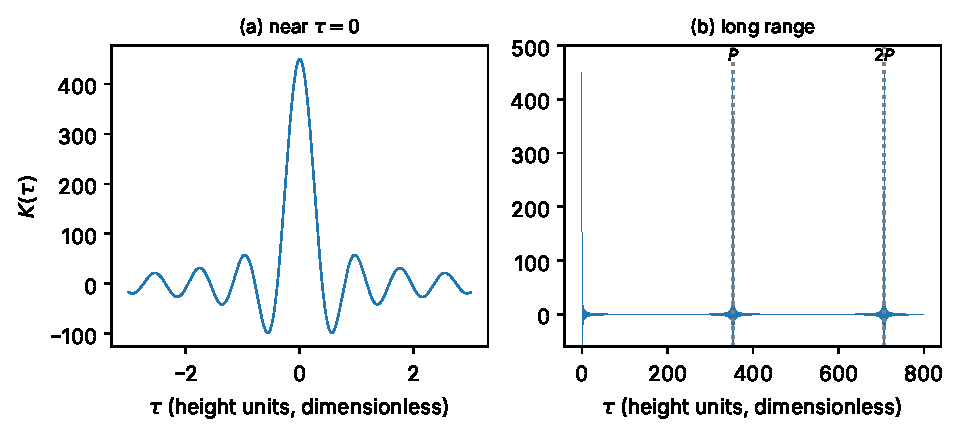
\includegraphics[width=0.85\linewidth]{figs/sparse-frequency_kernel.pdf}
\caption{The kernel $K(\tau)=\sum_{j=1}^{450}\cos(j\Delta\omega\,\tau)$ of the dense uniform-grid model C1, $\Delta\omega=8/450$. (a)~Near $\tau=0$: a narrow central peak of height 450 whose first zero lies at $\tau\approx0.39$ in $t$. (b)~Over a long range: the peak recurs at $\tau=P\approx353.4$, because every grid frequency is a multiple of $\Delta\omega$. By \eqref{eq:sparse-frequency-kernel}, the fitted C1 model at height $t$ is built from training values near $t$ and near its periodic images $t\pm P,\ t\pm2P,\dots$}
\label{fig:sparse-frequency-kernel}
\end{figure}

Put the two facts together. By \eqref{eq:sparse-frequency-kernel}, the C1 prediction at a held-out height $t$ is dominated by the training values $y_n$ at heights $t_n$ within a fraction of a unit of $t$, or of one of its images $t-P$, $t-2P$, and so on. Just beyond the training window there are no training zeros within a fraction of a unit; the nearest information is at the images, roughly $353$ or $707$ units earlier. Our interpretation of the kernel form (it is not an analysis given in the paper) is that C1 acts, in effect, as a \emph{local interpolator plus a periodic copying rule}; how strongly each part acts depends on the weights $\alpha_n$, which the ridge strength shrinks. It encodes no notion that a frequency found in the window should persist. That is the sense in which it "behaves like a generic basis": like the fitted potentials of Chapter~\ref{ch:generalization}, with 900 coefficients on 400 zeros it can fit anything in-sample, and outside it falls back on whatever its structure dictates, which here is local smoothing and repetition. Ridge regularization (chosen by forward validation) shrinks the $\alpha_n$, pulling $F$ toward zero, that is, toward the null.

\begin{sample}{The C1 grid compared with the window}
For the 400-zero training window, take its length as $T=t_{400}-t_1\approx666$. (a)~Compare the C1 grid spacing with the resolution $2\pi/T$. (b)~Which grid frequency lies nearest $\log2$, and by how much does it miss? (c)~How many periods of the $p=2$ wave fit into one period $P$ of the C1 model?

\textbf{Step 1: spacing and resolution.} $\Delta\omega=8/450=0.01778$. $2\pi/T=2\pi/666=0.0094$. The grid spacing is about $1.9$ resolution cells: the grid is \emph{coarser} than the window's resolution.

\textbf{Step 2: nearest to $\log2$.} $\log2/\Delta\omega=0.693147\times450/8=38.99$, so $j=39$ and $\omega_{39}=39\times8/450=0.693333$, which misses $\log 2=0.693147$ by $1.86\times10^{-4}$.

\textbf{Step 3: periods.} $P/(2\pi/\log2)=P\log2/(2\pi)=(450/8)\log2=38.99$.

$$\boxed{\Delta\omega\approx1.9\times\tfrac{2\pi}{T};\quad \omega_{39}=0.693333,\ \text{miss }1.86\times10^{-4};\quad P\ \text{holds}\ 38.99\ \text{periods of}\ \log2}$$
\end{sample}

The near-integer 38.99 is a coincidence of the paper's choice of grid: it means the $p=2$ wave very nearly repeats after one C1 period. This is our own observation, not an analysis in the paper; whether it contributes to C1's small positive held-out correlation ($+0.28$, interval $[+0.08,+0.46]$ in Table~IV) has not been checked, and Problem~6 invites you to explore it.

\begin{checkpoint}
A model uses only frequencies that are integer multiples of $\Delta\omega$. Can it represent a sinusoid of frequency $\log2$ accurately over an arbitrarily long stretch of $t$?
\end{checkpoint}
\checkanswer{No. The model is exactly periodic with period $2\pi/\Delta\omega$, while $\sin(t\log2)$ is periodic with period $2\pi/\log2$; unless $\log2$ were a rational multiple of $\Delta\omega$ the two drift apart, so any match on one stretch degrades on later stretches.}

\begin{pitfall}
"The dense grid contains frequencies near every $\log q$, so it contains the answer." Containing approximately the right frequencies is not enough: the fit must also \emph{prefer} them. With more coefficients than data, infinitely many coefficient vectors fit the window exactly (Chapter~\ref{ch:least-squares}), and the ridge solution picks the one of smallest norm, which spreads weight over all 450 frequencies rather than concentrating it on the few that are right.
\end{pitfall}

\begin{keyideas}
\item A sum of sinusoids on a uniform frequency grid of spacing $\Delta\omega$ is exactly periodic with period $2\pi/\Delta\omega$, \eqref{eq:sparse-frequency-period}; for C1 that period is about $353.4$.
\item The ridge fit of any linear model can be rewritten as a weighted sum of kernels centred at the training points, \eqref{eq:sparse-frequency-kernel}; for C1 the kernel is the Dirichlet kernel \eqref{eq:sparse-frequency-dirichlet}, narrow and periodic.
\item So C1 predicts by local interpolation and periodic copying: a generic basis with no preference for persistent frequencies. Its near-null score in Table~IV shows that capacity without a suitable prior does not generalize.
\end{keyideas}

%======================================================================
\section{Greedy sparse frequency search: control C2}\label{sec:sparse-frequency-greedy}

\subsection{The periodogram of irregular samples}

Control C2 is told only that a few sinusoids suffice. To find them it uses the tool of Chapter~\ref{ch:fourier-transform}: the periodogram. For values $r_n$ at irregular heights $t_n$, $n=1,\dots,n_{\rm fit}$, define
\begin{equation}
\mathcal P(\omega)=\frac{1}{n_{\rm fit}}\Bigl|\sum_{n}r_n\,e^{-\ii\omega t_n}\Bigr|^2
=\frac{1}{n_{\rm fit}}\Bigl[\Bigl(\sum_n r_n\cos\omega t_n\Bigr)^2+\Bigl(\sum_n r_n\sin\omega t_n\Bigr)^2\Bigr].
\label{eq:sparse-frequency-periodogram}
\end{equation}
The second form follows from $e^{-\ii\theta}=\cos\theta-\ii\sin\theta$ and $\abs{u-\ii v}^2=u^2+v^2$. (Other normalizations exist, for example one that divides by the squared norm of each sine and cosine column; the exact convention of the paper is in its archived code \cite{zenodo}. The peak positions, which are all we use, are nearly the same for well-spread samples.)

\begin{sample}{Height and width of a periodogram peak}
Let $r_n=A\cos(\omega_0t_n+\varphi)$ with $n_{\rm fit}=400$ samples spread over a window of length $T$, many periods long. Find $\mathcal P(\omega_0)$ for $A=0.225$ (the amplitude of the $p=2$ term, \cref{tab:sparse-frequency-amps}), and the offset $\delta$ at which $\mathcal P(\omega_0+\delta)$ first vanishes.

\textbf{Step 1: expand the sum at $\omega=\omega_0$.} Using $\cos\theta=\tfrac12(e^{\ii\theta}+e^{-\ii\theta})$,
$$r_ne^{-\ii\omega_0t_n}=\tfrac A2\bigl[e^{\ii\varphi}+e^{-\ii\varphi}e^{-2\ii\omega_0t_n}\bigr].$$

\textbf{Step 2: sum over $n$.} The first term adds to $\tfrac A2n_{\rm fit}e^{\ii\varphi}$. The second is a sum of unit-size phasors rotating at frequency $2\omega_0$. To see that it stays small, assume, as an idealization (the zeros are in fact denser at greater height), that the samples are equally spaced, $t_n=t_1+(n-1)\Delta$. Then, apart from the constant factor $e^{-2\ii\omega_0t_1}$ of modulus 1, the second sum is a geometric series with ratio $z=e^{-2\ii\omega_0\Delta}$, and
$$\Bigl|\sum_{n=1}^{n_{\rm fit}}z^{n-1}\Bigr|=\frac{\abs{1-z^{n_{\rm fit}}}}{\abs{1-z}}\le\frac{2}{2\abs{\sin(\omega_0\Delta)}}=\frac{1}{\abs{\sin(\omega_0\Delta)}},$$
using $\abs{1-z^{n_{\rm fit}}}\le2$ and $\abs{1-e^{\ii\theta}}=2\abs{\sin(\theta/2)}$ with $\theta=-2\omega_0\Delta$. The bound does not grow with $n_{\rm fit}$ (unless $\omega_0\Delta$ is close to a multiple of $\pi$), while the first term grows like $n_{\rm fit}$. For the irregular zeros we carry the same conclusion over as a heuristic. Neglecting the second term,
$\sum_nr_ne^{-\ii\omega_0t_n}\approx\tfrac A2n_{\rm fit}e^{\ii\varphi}$.

\textbf{Step 3: square.} $\mathcal P(\omega_0)\approx\frac{1}{n_{\rm fit}}\bigl(\tfrac A2n_{\rm fit}\bigr)^2=\frac{n_{\rm fit}A^2}{4}=\frac{400(0.225)^2}{4}=5.06.$

\textbf{Step 4: off the peak.} At $\omega=\omega_0+\delta$ the surviving term is $\tfrac A2e^{\ii\varphi}\sum_ne^{-\ii\delta t_n}$. Replace the sum by $(n_{\rm fit}/T)$ times the integral over the window, as in \eqref{eq:sparse-frequency-orth}. With $u=t-t_c$,
$$\frac1T\int_{t_c-T/2}^{t_c+T/2}e^{-\ii\delta t}\,\dd t=\frac{e^{-\ii\delta t_c}}{T}\int_{-T/2}^{T/2}e^{-\ii\delta u}\,\dd u=\frac{e^{-\ii\delta t_c}}{T}\,\frac{e^{-\ii\delta T/2}-e^{\ii\delta T/2}}{-\ii\delta}=e^{-\ii\delta t_c}\,\frac{\sin(\delta T/2)}{\delta T/2},$$
where the last step uses $e^{-\ii a}-e^{\ii a}=-2\ii\sin a$ with $a=\delta T/2$. Since $\abs{e^{-\ii\delta t_c}}=1$, the magnitude of the surviving term is $\tfrac A2n_{\rm fit}\abs{\sin(\delta T/2)/(\delta T/2)}$, so
\begin{equation}
\mathcal P(\omega_0+\delta)\approx\frac{n_{\rm fit}A^2}{4}\left[\frac{\sin(\delta T/2)}{\delta T/2}\right]^2 ,
\label{eq:sparse-frequency-peak}
\end{equation}
which first vanishes when $\delta T/2=\pi$.

$$\boxed{\mathcal P(\omega_0)\approx n_{\rm fit}A^2/4\approx5.06,\qquad \text{first zero at }\delta=2\pi/T}$$
\end{sample}

So a sinusoid of amplitude $A$ produces a peak of height proportional to $A^2$, centred at its frequency, with width set by the window. The largest peak belongs to the largest-amplitude sinusoid, provided the peaks are separated by more than their widths.

\begin{figure}[htbp]\centering
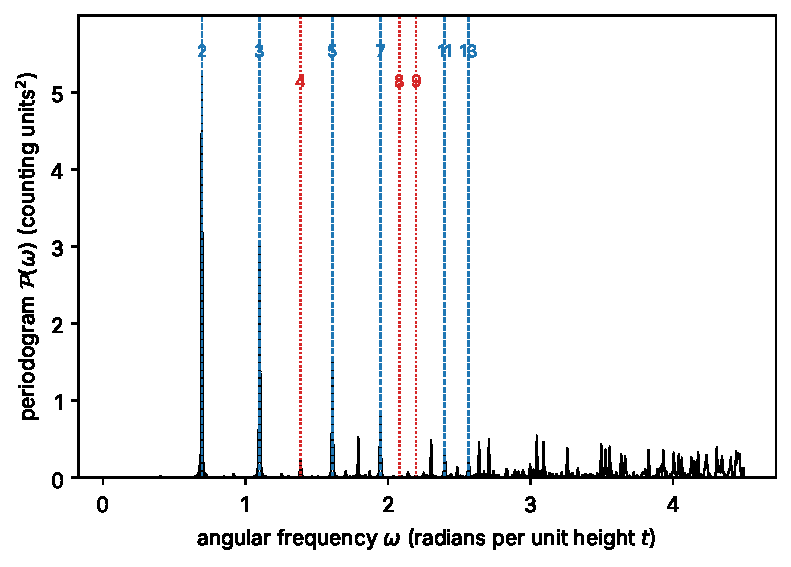
\includegraphics[width=0.85\linewidth]{figs/sparse-frequency_periodogram.pdf}
\caption{Periodogram \eqref{eq:sparse-frequency-periodogram} of the targets $y_n=n-\tfrac12-\Nsm(t_n)$ for the first 400 zeros, for $0.05<\omega<4.5$. Dashed lines mark $\log p$ for primes $p\le13$ (labelled); dotted lines mark the squares and cubes $\log4,\log8,\log9$. The zeros were never told these frequencies; compare the positions of the tallest peaks with the marked lines. The peak widths are of order $2\pi/T\approx0.0094$.}
\label{fig:sparse-frequency-periodogram}
\end{figure}

\subsection{The greedy algorithm}

Control C2 builds its model one frequency at a time (paper Sec.~II~D; Appendix~A step~(20)):
\begin{enumerate}
\item Start with the residual equal to the data, $\bm r^{(0)}=\bm y$, and an empty frequency list.
\item \textbf{Search.} Compute the periodogram of the current residual on a coarse grid covering $0.05<\omega<8$, with step a quarter of the resolution, $\tfrac14\cdot2\pi/T$. Take the grid point with the largest value.
\item \textbf{Refine.} Recompute the periodogram on a fine grid of 201 points around that coarse peak and take the maximum. (The record gives the count, 201; in our listings we take the fine grid to span one coarse step on each side, a natural reading; the exact span is in the archived code.)
\item \textbf{Refit jointly.} Append the refined frequency to the list and refit \emph{all} amplitudes $a_j,b_j$ of the chosen frequencies together by ridge least squares, \eqref{eq:sparse-frequency-ridge}.
\item \textbf{Update.} Set the new residual $\bm r=\bm y-X\bm c$ and return to step 2, until $K$ frequencies have been chosen.
\end{enumerate}
Each chosen frequency contributes three fitted numbers: $\omega_j$ (chosen by the search) and $a_j,b_j$. A model with $K$ frequencies has $3K$ parameters, which is why Table~IV lists C2 with "72, 129" parameters for $K=24$ and $K=43$.

Why does the search never pick the same frequency twice? After a plain least-squares refit, the residual is orthogonal to every column of $X$ (Chapter~\ref{ch:least-squares}: $X^\top(\bm y-X\bm c)=\bm 0$ is the normal equation \eqref{eq:sparse-frequency-normal} rearranged). The columns include $\cos\omega_jt_n$ and $\sin\omega_jt_n$ for each chosen $\omega_j$, so both sums in \eqref{eq:sparse-frequency-periodogram} vanish and $\mathcal P(\omega_j)=0$ there. With a small ridge the orthogonality is approximate, and the periodogram is nearly zero at chosen frequencies.

\begin{sample}{How much peak can the coarse grid miss?}
The coarse grid step is $\tfrac14\cdot2\pi/T$. In the worst case the true peak lies halfway between grid points. By what factor is the periodogram there reduced relative to the true peak height, and why is the refinement step worth having?

\textbf{Step 1: worst offset.} Half a coarse step: $\delta=\tfrac18\cdot\frac{2\pi}{T}=\frac{\pi}{4T}$.

\textbf{Step 2: sinc argument.} $\delta T/2=\pi/8=0.3927$.

\textbf{Step 3: apply \eqref{eq:sparse-frequency-peak}.} $\sin(\pi/8)/(\pi/8)=0.38268/0.39270=0.9745$; squared, $0.9496$.

\textbf{Step 4: interpret.} The coarse grid sees at least about 95\% of every peak, so it rarely misses a strong one, but two peaks whose heights differ by less than about 5\% could be ranked in the wrong order, and the coarse frequency can be off by up to $\pi/(4T)$. The refinement pins the frequency down much more finely than the coarse step before it is frozen into the model, which matters because frequency errors grow into phase errors outside the window (\cref{sec:sparse-frequency-precision}).

$$\boxed{\text{worst-case peak height}\approx0.9745^2\approx0.950\ \text{of the true peak}}$$
\end{sample}

\begin{pycode}
def periodogram(tt, r, w):
    C = np.cos(np.outer(w, tt)); S = np.sin(np.outer(w, tt))
    return ((C @ r)**2 + (S @ r)**2) / len(tt)

def greedy(tt, yy, K, lam=1e-8):
    T = tt[-1] - tt[0]
    step = 0.25*2*np.pi/T                        # quarter of the resolution
    coarse = np.arange(0.05, 8.0, step)
    om, r = [], yy.copy()
    for k in range(K):
        w0 = coarse[np.argmax(periodogram(tt, r, coarse))]
        fine = np.linspace(w0 - step, w0 + step, 201)
        om.append(fine[np.argmax(periodogram(tt, r, fine))])
        X = design(tt, np.array(om))             # joint refit of all amplitudes
        U, s, Vt = np.linalg.svd(X, full_matrices=False)
        c = Vt.T @ (s/(s**2 + lam*s[0]**2) * (U.T @ yy))
        r = yy - X @ c
    return np.array(om), c

om24, c24 = greedy(t[:400], y[:400], 24)
print(np.round(om24[:5], 4), np.log([2, 3, 5]))
\end{pycode}

If you run this listing, the first frequency chosen lies within $\pi/T$ of $\log2=0.6931$: the largest peak of the zeros' fluctuation is the dominant term of running example RE2.

\subsection{Matching pursuit: the general idea}

The greedy search is an instance of a general method called \textbf{matching pursuit}. You have a \emph{dictionary} of candidate shapes (here: sinusoids of every frequency in the band), and you build an approximation of the data by repeatedly picking the dictionary element that best matches the current residual. Two variants:
\begin{itemize}
\item \emph{Plain matching pursuit}: pick the element most aligned with the residual, add its projection, keep all earlier coefficients frozen.
\item \emph{Orthogonal matching pursuit}: pick the element the same way, then refit \emph{all} chosen coefficients jointly by least squares. This is what C2 does.
\end{itemize}
Each element of the dictionary is called an \textbf{atom}. The two samples below work in tiny dimensions: the first shows the orthonormal case, where plain and orthogonal pursuit agree; the second shows, with overlapping atoms, why the joint refit matters.

\begin{sample}{Matching pursuit with an orthonormal dictionary}
In four dimensions take the orthonormal dictionary $\bm d_1=\tfrac12(1,1,1,1)$, $\bm d_2=\tfrac12(1,-1,1,-1)$, $\bm d_3=\tfrac1{\sqrt2}(1,0,-1,0)$, $\bm d_4=\tfrac1{\sqrt2}(0,1,0,-1)$, and data $\bm y=(3,1,-1,1)$. Run matching pursuit.

\textbf{Step 1: inner products with the data.} $\bm y\cdot\bm d_1=\tfrac12(3+1-1+1)=2$; $\bm y\cdot\bm d_2=\tfrac12(3-1-1-1)=0$; $\bm y\cdot\bm d_3=\tfrac{1}{\sqrt2}(3+1)=2.828$; $\bm y\cdot\bm d_4=\tfrac1{\sqrt2}(1-1)=0$.

\textbf{Step 2: first pick.} The largest is $\bm d_3$, coefficient $2.828$. Residual: $\bm y-2.828\,\bm d_3=(3,1,-1,1)-(2,0,-2,0)=(1,1,1,1)$.

\textbf{Step 3: second pick.} $\bm r\cdot\bm d_1=2$, all others zero. Add $2\bm d_1=(1,1,1,1)$; the residual is now $\bm 0$.

\textbf{Step 4: compare with joint refit.} Because the dictionary is orthonormal, the coefficient of each element does not change when others are added, so plain and orthogonal pursuit agree.

$$\boxed{\bm y=2.828\,\bm d_3+2\,\bm d_1\ \text{(two atoms, exact)}}$$
\end{sample}

\begin{sample}{Why the joint refit matters}
In the plane take unit vectors $\bm a=(1,0)$ and $\bm b=(\cos60^\circ,\sin60^\circ)=(0.5,0.866)$, and data $\bm y=\bm a+0.8\,\bm b=(1.4,0.6928)$. Run two steps of plain matching pursuit, then orthogonal matching pursuit.

\textbf{Step 1: first pick.} $\bm y\cdot\bm a=1.4$, $\bm y\cdot\bm b=1.4(0.5)+0.6928(0.866)=0.7+0.6=1.3$. Pick $\bm a$ with coefficient $1.4$ (not the true $1$). Residual $\bm r=(0,0.6928)$.

\textbf{Step 2 (plain): second pick.} $\bm r\cdot\bm b=0.6928(0.866)=0.6$. Add $0.6\,\bm b$, keeping $1.4$ on $\bm a$. Approximation $1.4\,\bm a+0.6\,\bm b=(1.7,0.5196)$; residual $(-0.3,0.1732)$, length $\sqrt{0.09+0.03}=0.346$.

\textbf{Step 2 (orthogonal): refit both.} Solve $\alpha\bm a+\beta\bm b=\bm y$: the second component gives $0.866\beta=0.6928$, so $\beta=0.8$; the first gives $\alpha+0.5(0.8)=1.4$, so $\alpha=1$. Residual $\bm 0$.

\textbf{Step 3: interpret.} When dictionary elements overlap, the first coefficient is contaminated by the part of the data that belongs to elements not yet chosen. Freezing it leaves a permanent error; the joint refit removes it. Nearby frequencies overlap in exactly this way when they are within a few resolution cells, \eqref{eq:sparse-frequency-orth}.

$$\boxed{\text{plain: }(1.4,0.6),\ \text{residual }0.346;\quad \text{orthogonal: }(1,0.8),\ \text{residual }0}$$
\end{sample}

\begin{figure}[htbp]\centering
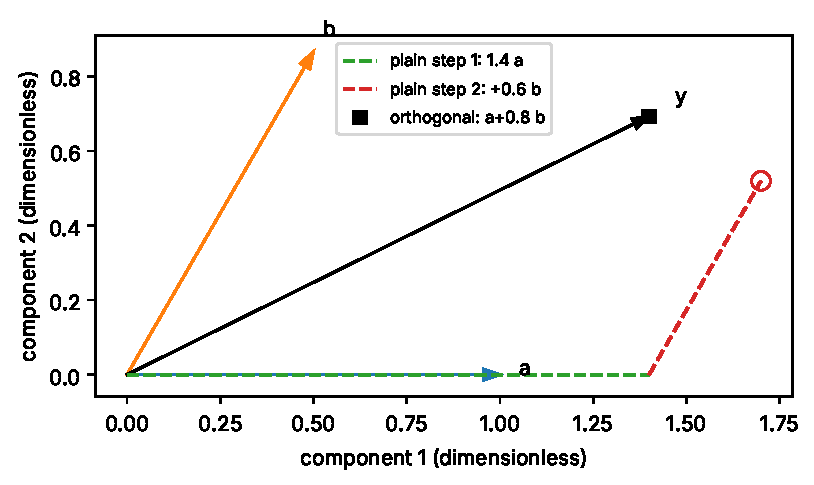
\includegraphics[width=0.75\linewidth]{figs/sparse-frequency_pursuit.pdf}
\caption{Plain versus orthogonal matching pursuit for the vectors of the sample above. The data $\bm y=\bm a+0.8\bm b$ (black). Plain pursuit takes the projection $1.4\,\bm a$ onto $\bm a$, then adds the projection of the residual onto $\bm b$, ending at $1.4\,\bm a+0.6\,\bm b$ (open circle) with a leftover error. Orthogonal pursuit refits both coefficients jointly and lands exactly on $\bm y$.}
\label{fig:sparse-frequency-pursuit}
\end{figure}

\begin{beyond}
When does greedy selection provably find the right few elements? For dictionaries whose elements are nearly orthogonal and signals that are truly sparse, there are theorems (from the field called sparse approximation or compressed sensing) guaranteeing that orthogonal matching pursuit recovers the correct elements; they require bounds on the overlaps between elements and on the noise. Those theorems are beyond this book, and we do not claim that their hypotheses hold for the zeros. For C2 the evidence that the right frequencies were found is empirical: they land at $\log q$ (\cref{sec:sparse-frequency-primes}) and they predict held-out zeros.
\end{beyond}

\begin{pitfall}
Aliasing. For samples equally spaced by $\Delta$, frequencies above $\pi/\Delta$ are indistinguishable from lower ones (Chapter~\ref{ch:fourier-transform}). The mean spacing of the zeros at the top of the 400-zero window is about $1.34$, giving $\pi/1.34\approx2.34$, yet the paper's band reaches $\omega=8$ and the 800-zero search recovered frequencies above $\log131\approx4.88$. This is not a contradiction: the zeros are irregular samples whose mean spacing shrinks severalfold across the window (Chapter~\ref{ch:counting-zeros}), so an alias that matches the samples at one height fails at another. Do not carry rules for uniform sampling over to irregular sampling without thought; equally, do not assume irregular sampling removes all ambiguity.
\end{pitfall}

\begin{checkpoint}
Before any frequency is chosen, which frequency do you expect the greedy search to pick first for the zeros, and why?
\end{checkpoint}
\checkanswer{$\log2$. The periodogram peak height grows like the square of the amplitude, and among the terms of \eqref{eq:sparse-frequency-nfl} the $p=2$, $m=1$ term has the largest amplitude, $1/(\pi\sqrt2)=0.225$ (\cref{tab:sparse-frequency-amps}).}

\begin{keyideas}
\item A sinusoid of amplitude $A$ gives a periodogram peak of height about $n_{\rm fit}A^2/4$ and width $2\pi/T$, \eqref{eq:sparse-frequency-peak}.
\item Control C2: repeatedly take the largest periodogram peak of the residual (coarse grid of step $\tfrac14\cdot2\pi/T$, then refinement), and refit all amplitudes jointly; $K$ frequencies cost $3K$ parameters.
\item This is orthogonal matching pursuit. Joint refitting matters when dictionary elements overlap, as nearby frequencies do.
\end{keyideas}

%======================================================================
\section{Choosing $K$ and the ridge: forward validation}\label{sec:sparse-frequency-validation}

The greedy search can go on adding frequencies until it fits the training data perfectly. Training error can only fall as $K$ grows: each model contains the previous one (set the new amplitudes to zero), so the least-squares minimum cannot rise. Chapter~\ref{ch:generalization} told you that this proves nothing about prediction. We need a rule for stopping that uses only training data.

The paper's rule (Sec.~II~D): split the training window \emph{forward}. Fit on the first 75\% of the training zeros, score on the last 25\%, choose the ridge strength $\lambda$ and the number of frequencies $K$ that score best on that last quarter, and finally refit the chosen configuration on the whole training window. Held-out zeros are never touched before scoring.

Why forward and not a random quarter? Because the real task is forward extrapolation: predicting zeros above the window. A validation split should imitate the task. A random split would place validation zeros between training zeros, where a model can score well by interpolating neighbours, which says little about extrapolation; and, as Chapter~\ref{ch:generalization} showed, the serial correlation of the fluctuations makes interpolation behave quite differently from extrapolation.

The record (Appendix~A step~(20)) adds that the procedure was checked for leakage directly: overwriting the held-out data with noise before fitting leaves all fitted coefficients bit-identical. This is a cheap and decisive test you can apply to any pipeline: if the fit changes when held-out data are corrupted, held-out data are leaking into the fit.

\begin{sample}{The bookkeeping of the validation search}
For training windows of 400 and 800 zeros, find (a) the sizes of the inner fit and validation sets, (b) the number of ridge strengths in the paper's grid $\lambda=10^{-8},\dots,10^{3}$ in half decades, (c) the cap on $K$ from the rule $K\le\min(300,n_{\rm fit}/3)$, and (d) the approximate number of coarse search frequencies on $0.05<\omega<8$ for each window, taking $T\approx666$ and $T\approx1170$.

\textbf{Step 1: split.} $0.75\times400=300$ fit, $100$ validate; $0.75\times800=600$ fit, $200$ validate.

\textbf{Step 2: ridge grid.} The exponents run $-8,-7.5,\dots,3$, a span of $11$ decades in steps of $0.5$: $11/0.5+1=23$ values.

\textbf{Step 3: cap on $K$.} $n_{\rm fit}/3=133.3$ for 400 zeros, so $K\le133$; $800/3=266.7$, so $K\le266$; both are below 300. The cap keeps $3K\le n_{\rm fit}$: never more parameters than data.

\textbf{Step 4: coarse grid size.} Step $\tfrac14\cdot2\pi/T$. Number of points $\approx7.95/(\tfrac14\cdot2\pi/T)=7.95\times4T/(2\pi)$: for $T\approx666$ about $3{,}400$; for $T\approx1170$ about $5{,}900$.

$$\boxed{300/100\ \text{and}\ 600/200;\ 23\ \text{ridge values};\ K\le133\ \text{and}\ K\le266;\ \approx3{,}400\ \text{and}\ \approx5{,}900\ \text{coarse frequencies}}$$
\end{sample}

How should you search over $K$ efficiently? One run of the greedy algorithm on the inner 75\% up to the cap produces the whole nested sequence of models with $K=1,2,3,\dots$; you can score each on the validation quarter as you go. (This is our suggestion for an implementation, not a statement about the paper's code.) The paper's validation selected $K=24$ for the 400-zero window and $K=43$ for the 800-zero window (Sec.~IV; Appendix~A, revision anchors).

\begin{figure}[htbp]\centering
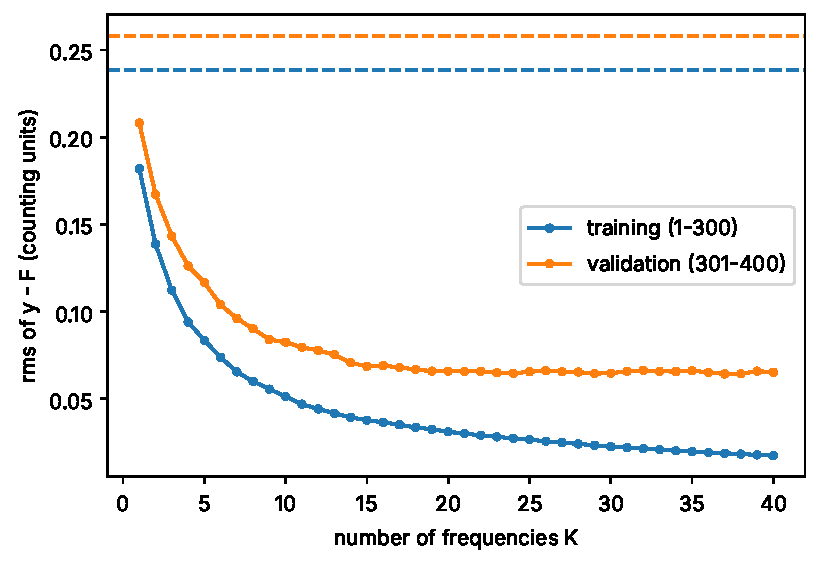
\includegraphics[width=0.85\linewidth]{figs/sparse-frequency_greedy.pdf}
\caption{Greedy sparse search inside the 400-zero training window, split forward: inner fit on zeros 1--300, validation on 301--400. Training rms (filled) and validation rms (open) of $y_n-F(t_n)$, in counting units, against the number of frequencies $K$; dashed lines show the null (predicting $F=0$) on each set. The training error can only fall, because the models are nested; the validation error is what selects $K$. Here the validation error is measured on $y_n$ at the true zeros, a simplification of the paper's scoring through root solving (by \eqref{eq:sparse-frequency-errorlink} the two agree to first order).}
\label{fig:sparse-frequency-greedy}
\end{figure}

\begin{checkpoint}
A colleague selects $K$ by scoring on a random 25\% of the training zeros instead of the last 25\%. Why might the chosen $K$ be poorly suited to predicting zeros above the window?
\end{checkpoint}
\checkanswer{Random validation zeros sit between training zeros, so the score rewards models that interpolate well locally; that need not be the same $K$ that extrapolates well. A forward split tests the model on the kind of task it will face: values beyond the data it was fitted on.}

\begin{keyideas}
\item Training error never rises with $K$; the choice of $K$ and ridge must come from data the inner fit did not see.
\item The paper uses a forward 75/25 split inside the training window, a 23-value ridge grid, and $K\le\min(300,n_{\rm fit}/3)$, then refits on the whole window. Held-out zeros are untouched, as checked by overwriting them with noise.
\end{keyideas}

%======================================================================
\section{How well can a frequency be learned? Resolution, precision and dephasing}\label{sec:sparse-frequency-precision}

\subsection{Resolution is not precision}

Recall from Chapter~\ref{ch:fourier-transform} that a window of length $T$ has resolution $2\pi/T$: two frequencies closer than that blur into one peak. Resolution is about \emph{separating} two frequencies. Precision is about \emph{locating} one isolated frequency, and it can be much better than the resolution, because the centre of a well-measured peak can be found far more accurately than its width. Here is a linearized least-squares estimate of how well.

\subsection{Deriving the precision}

\emph{Model and assumptions.} Measure time from the window centre, $u_n=t_n-t_c$, and suppose
\begin{equation}
y_n=A\sin(\omega u_n+\varphi)+e_n ,
\end{equation}
where the $e_n$ are independent errors of mean zero and variance $\sigma^2$ (for the zeros, "error" is everything other than the one sinusoid we are estimating, which is not truly independent noise: so what follows is a heuristic scale, not a rigorous bound). Suppose the samples are spread roughly uniformly over the window and $A$ and $\varphi$ are known well. We want the uncertainty in $\omega$.

\emph{Step 1: linearize.} Near the true frequency $\omega_0$, write $\omega=\omega_0+\delta\omega$ and expand to first order (Chapter~\ref{ch:asymptotics}):
\begin{equation}
A\sin\bigl((\omega_0+\delta\omega)u_n+\varphi\bigr)\approx A\sin(\omega_0u_n+\varphi)+g_n\,\delta\omega,
\qquad g_n=A\,u_n\cos(\omega_0u_n+\varphi).
\end{equation}

\emph{Step 2: one-parameter least squares.} Fitting $\delta\omega$ to the data $d_n=y_n-A\sin(\omega_0u_n+\varphi)$ means minimizing $\sum_n(d_n-g_n\delta\omega)^2$. Setting the derivative with respect to $\delta\omega$ to zero, $-2\sum_ng_n(d_n-g_n\delta\omega)=0$, so
\begin{equation}
\widehat{\delta\omega}=\frac{\sum_ng_nd_n}{\sum_ng_n^2}.
\end{equation}

\emph{Step 3: its variance.} At the true frequency, $d_n=e_n$. A sum $\sum_n w_ne_n$ of independent errors with fixed weights has variance $\sigma^2\sum_nw_n^2$ (Chapter~\ref{ch:probability}). With $w_n=g_n/\sum_mg_m^2$,
\begin{equation}
\mathrm{Var}\bigl(\widehat{\delta\omega}\bigr)=\sigma^2\frac{\sum_ng_n^2}{\bigl(\sum_ng_n^2\bigr)^2}=\frac{\sigma^2}{\sum_ng_n^2}.
\end{equation}

\emph{Step 4: evaluate $\sum g_n^2$.} Using $\cos^2\theta=\tfrac12(1+\cos2\theta)$,
\begin{equation}
\sum_ng_n^2=A^2\sum_nu_n^2\cos^2(\omega_0u_n+\varphi)=\frac{A^2}{2}\sum_nu_n^2+\frac{A^2}2\sum_nu_n^2\cos\bigl(2(\omega_0u_n+\varphi)\bigr).
\end{equation}
The second sum oscillates and is small compared with the first when the window holds many periods. For samples spread uniformly over $[-T/2,T/2]$, the average of $u^2$ is $\frac1T\int_{-T/2}^{T/2}u^2\,\dd u=\frac{T^2}{12}$, so $\sum_nu_n^2\approx n\,T^2/12$ with $n$ the number of samples. Hence $\sum_ng_n^2\approx A^2nT^2/24$.

\emph{Step 5: why the phase does not interfere.} If $\varphi$ is fitted too, linearize in both parameters: the model changes by $g_n\,\delta\omega+h_n\,\delta\varphi$ with $h_n=A\cos(\omega_0u_n+\varphi)$. Least squares for $(\delta\omega,\delta\varphi)$ then gives the $2\times2$ normal equations
\begin{equation}
\begin{pmatrix}\sum_ng_n^2&\sum_ng_nh_n\\ \sum_ng_nh_n&\sum_nh_n^2\end{pmatrix}\begin{pmatrix}\delta\omega\\ \delta\varphi\end{pmatrix}=\begin{pmatrix}\sum_ng_nd_n\\ \sum_nh_nd_n\end{pmatrix}.
\end{equation}
The off-diagonal entry is $\sum_ng_nh_n=A^2\sum_nu_n\cos^2(\omega_0u_n+\varphi)=\tfrac{A^2}{2}\sum_nu_n+\tfrac{A^2}{2}\sum_nu_n\cos\bigl(2(\omega_0u_n+\varphi)\bigr)$. The first sum is close to zero because $u$ is measured from the window centre, so positive and negative $u_n$ cancel; the second oscillates and is small compared with the diagonal entries. Neglecting the off-diagonal entry, the matrix is diagonal, and its first row reads $\bigl(\sum_ng_n^2\bigr)\delta\omega=\sum_ng_nd_n$, exactly the one-parameter equation of Step 2. The variance of Step 3 is therefore unchanged. The two parameters decouple, which is why we centred the time variable.

\emph{Result.}
\begin{equation}
\mathrm{std}(\widehat\omega)\approx\frac{\sqrt{24}\,\sigma}{A\sqrt n\,T}.
\label{eq:sparse-frequency-varomega}
\end{equation}
Two lessons. The precision improves like $1/T$ with the window length and like $1/\sqrt n$ with the number of samples; and it is worse for weak components (small $A$), which is why the greedy search places weak frequencies less accurately than strong ones.

\begin{beyond}
Equation \eqref{eq:sparse-frequency-varomega} has the form of the Cram\'er--Rao lower bound for estimating the frequency of a sinusoid in independent Gaussian noise, a theorem from statistical estimation theory that bounds the variance of any unbiased estimator. Its proof and the precise conditions are beyond this book; for least-squares estimation more generally see \cite{nr} or \cite{esl}. For the zeros the "noise" is the deterministic sum of all other sinusoids, so treat \eqref{eq:sparse-frequency-varomega} only as an order-of-magnitude scale.
\end{beyond}

\begin{sample}{Precision of the learned $\log 2$}
Estimate the precision of the $p=2$ frequency learned from 400 zeros, taking $A=0.225$ (\cref{tab:sparse-frequency-amps}), $\sigma=0.18$ (an illustrative rms for everything else in $y$; the full fluctuation of zeros 1--400 has rms $0.2438$ according to the paper's Appendix~A anchors), $n=400$ and $T=666$. Compare with the resolution $2\pi/T$ and the matching tolerance $\pi/T$.

\textbf{Step 1: numerator.} $\sqrt{24}\,\sigma=4.899\times0.18=0.8818$.

\textbf{Step 2: denominator.} $A\sqrt n\,T=0.225\times20\times666=2997$.

\textbf{Step 3: divide.} $\mathrm{std}(\widehat\omega)\approx0.8818/2997=2.94\times10^{-4}$.

\textbf{Step 4: compare.} $2\pi/T=0.00943$, so the precision is about $3\%$ of a resolution cell. $\pi/T=0.00472$, about 16 times larger than the estimated error.

$$\boxed{\mathrm{std}(\widehat\omega)\approx2.9\times10^{-4},\ \text{about }0.031\ \text{resolution cells, }1/16\ \text{of }\pi/T}$$
\end{sample}

\begin{checkpoint}
If the number of training zeros doubles from 400 to 800, the window grows from $T\approx666$ to $T\approx1170$. If $A$ and $\sigma$ stayed the same, by what factor would \eqref{eq:sparse-frequency-varomega} improve?
\end{checkpoint}
\checkanswer{By $\sqrt2\times(1170/666)\approx2.5$: a factor $\sqrt2$ from the number of samples and a factor $1170/666$ from the window length.}

\subsection{Dephasing: why skill decays far from the window}

A learned frequency is never exactly right. Inside the window the fit compensates: the fitted phase is correct near the window centre, and the error of the phase stays small across the window. Outside, there is nothing to compensate.

\emph{Setup.} Let the true component be $A\sin\theta$ with $\theta=\omega_0(t-t_c)+\varphi$, and the fitted one $A\sin(\theta+\phi)$ with the same amplitude and a frequency error $\delta\omega$. The phase error is then
\begin{equation}
\phi(t)=\delta\omega\,(t-t_c),
\label{eq:sparse-frequency-dephase}
\end{equation}
growing linearly with the distance $\Delta t=t-t_c$ from the window centre.

\emph{Prediction error.} Over a stretch of $t$ short enough that $\phi$ is nearly constant but long enough to contain many periods, $\theta$ sweeps uniformly through all angles. The difference between prediction and truth is
\begin{equation}
A\sin(\theta+\phi)-A\sin\theta=2A\cos\bigl(\theta+\tfrac\phi2\bigr)\sin\tfrac\phi2\quad\text{($\sin\alpha-\sin\beta=2\cos\tfrac{\alpha+\beta}2\sin\tfrac{\alpha-\beta}2$)}.
\end{equation}
The mean of $\cos^2$ over all angles is $\tfrac12$, so the mean square error is $4A^2\sin^2(\phi/2)\cdot\tfrac12$, and
\begin{equation}
\text{rms error}=\sqrt2\,A\,\abs{\sin(\phi/2)} .
\end{equation}
The null prediction (zero) has rms error equal to the rms of $A\sin\theta$, which is $A/\sqrt2$. The ratio is
\begin{equation}
\frac{\text{rms error}}{\text{null rms}}=2\abs{\sin(\phi/2)} .
\label{eq:sparse-frequency-rmsratio}
\end{equation}

\emph{Correlation.} The mean of $\sin\theta\sin(\theta+\phi)=\tfrac12[\cos\phi-\cos(2\theta+\phi)]$ over all angles is $\tfrac12\cos\phi$; each factor alone has mean square $\tfrac12$ and mean zero. Dividing the covariance by the product of the standard deviations (Chapter~\ref{ch:probability}),
\begin{equation}
\corr=\frac{\tfrac12A^2\cos\phi}{\sqrt{\tfrac12A^2}\sqrt{\tfrac12A^2}}=\cos\phi .
\label{eq:sparse-frequency-corr}
\end{equation}

\emph{Consequences.} At $\phi=0$ the prediction is perfect. As $\phi$ grows, the correlation falls as $\cos\phi$ and the error grows. The prediction is worse than the null once $2\abs{\sin(\phi/2)}>1$, that is, once $\phi>\pi/3$; at $\phi=\pi/2$ the correlation is zero; at $\phi=\pi$ the prediction is anticorrelated and twice as bad as the null. A model with many learned frequencies, each with its own small error, loses skill gradually, the weakest (least precise) components first.

\begin{sample}{How far does a learned frequency carry?}
A component is learned with frequency error $\delta\omega=3\times10^{-4}$, about the size found in the previous sample. (a)~At a distance $\Delta t=2000$ from the window centre, find the phase error, the rms ratio \eqref{eq:sparse-frequency-rmsratio} and the correlation. (b)~At what distance does this component's prediction become worse than the null?

\textbf{Step 1: phase.} $\phi=3\times10^{-4}\times2000=0.6$~rad.

\textbf{Step 2: rms ratio.} $2\sin(0.3)=2(0.2955)=0.591$.

\textbf{Step 3: correlation.} $\cos0.6=0.825$.

\textbf{Step 4: break-even.} $\phi=\pi/3$ requires $\Delta t=(\pi/3)/(3\times10^{-4})=3491$.

$$\boxed{\phi=0.6,\ \text{rms ratio}\approx0.59,\ \corr\approx0.83;\quad \text{worse than null beyond }\Delta t\approx3490}$$
\end{sample}

For the 400-zero window the centre is near $t_c\approx(14+680)/2=347$, and zero 2000 sits near $t\approx2515$ (values computed with \texttt{qmnt.zeros}), about $2170$ units away. So by \eqref{eq:sparse-frequency-dephase}, frequency errors of a few times $10^{-4}$ already cost a noticeable fraction of the skill on zeros 1001--2000. This is consistent with what the paper reports for C2 (Sec.~IV): from the 400-zero fit, $0.034$/$+0.99$ on zeros 401--500 but $0.078$/$+0.96$ on zeros 1001--2000, "as the estimated frequencies dephase, which the exact frequencies of the oracle do not". The oracle's exact frequencies have $\delta\omega=0$, so its relative skill stays nearly constant through zero $10^4$ (Table~V). Our single-sinusoid model is a picture of the mechanism, not a fit to the paper's numbers.

\begin{figure}[htbp]\centering
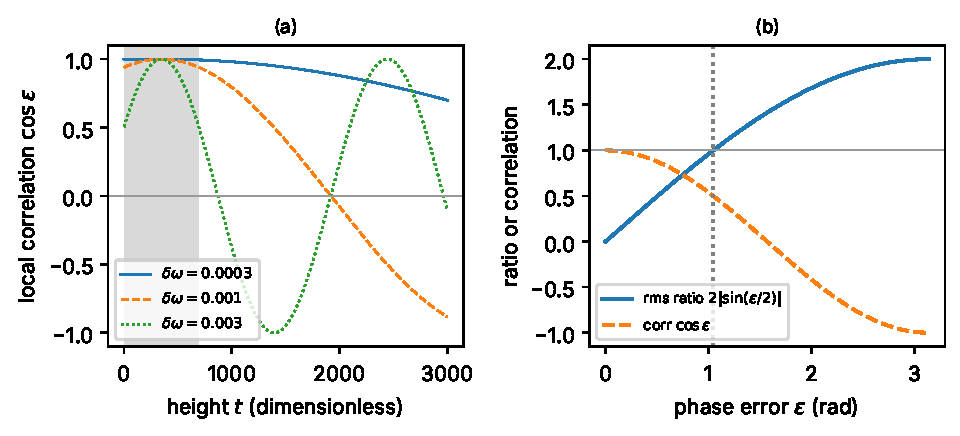
\includegraphics[width=\linewidth]{figs/sparse-frequency_dephasing.pdf}
\caption{Dephasing. (a)~Local correlation $\cos\phi(t)$ of a learned component with the truth, \eqref{eq:sparse-frequency-dephase} and \eqref{eq:sparse-frequency-corr}, for frequency errors $\delta\omega=3\times10^{-4}$, $10^{-3}$ and $3\times10^{-3}$; the 400-zero training window $14\le t\le680$ is shaded and $t$ is the height (dimensionless). (b)~Rms error relative to the null, $2\abs{\sin(\phi/2)}$, and correlation $\cos\phi$, against the phase error $\phi$; the prediction is worse than the null beyond $\phi=\pi/3$ (dotted).}
\label{fig:sparse-frequency-dephasing}
\end{figure}

\begin{keyideas}
\item Resolution ($2\pi/T$) limits separating frequencies; precision of a single strong frequency is much finer, roughly $\sqrt{24}\,\sigma/(A\sqrt n\,T)$, \eqref{eq:sparse-frequency-varomega}, a heuristic scale for the zeros.
\item A frequency error $\delta\omega$ becomes a phase error $\delta\omega\,\Delta t$ that grows with distance from the window, \eqref{eq:sparse-frequency-dephase}; correlation falls as $\cos\phi$, and the prediction is worse than the null beyond $\phi=\pi/3$.
\item Learned frequencies therefore lose skill far from the window; exact arithmetic frequencies do not.
\end{keyideas}

%======================================================================
\section{Recovering $\log p^m$ from the zeros}\label{sec:sparse-frequency-primes}

\subsection{What the zeros contain}

The truncated formula \eqref{eq:sparse-frequency-nfl} stops at $m=3$, but the formal series of Chapter~\ref{ch:explicit-formula} runs over all $m\ge1$. A term with prime power $q=p^m$ has frequency $\log q$ and amplitude
\begin{equation}
B_q=\frac{1}{\pi\,m\,p^{m/2}}=\frac{1}{\pi\,m\sqrt q}=\frac{\Lambda(q)}{\pi\log q\,\sqrt q},
\label{eq:sparse-frequency-amp}
\end{equation}
where the last form uses the von Mangoldt function of Chapter~\ref{ch:primes}, $\Lambda(p^m)=\log p$, so that $\Lambda(q)/\log q=\log p/(m\log p)=1/m$. \Cref{tab:sparse-frequency-amps} lists the strongest terms.

\begin{table}[htbp]\centering
\caption{Frequencies and amplitudes \eqref{eq:sparse-frequency-amp} of the first prime powers $q=p^m$ in the fluctuation of the counting function (counting units). Terms with $m\ge4$ are absent from the truncation \eqref{eq:sparse-frequency-nfl} but present in the zeros.}
\label{tab:sparse-frequency-amps}
\begin{tabular}{rccc}
\toprule
$q$ & $(p,m)$ & $\log q$ & $B_q$\\
\midrule
2 & (2,1) & 0.6931 & 0.2251\\
3 & (3,1) & 1.0986 & 0.1838\\
4 & (2,2) & 1.3863 & 0.0796\\
5 & (5,1) & 1.6094 & 0.1424\\
7 & (7,1) & 1.9459 & 0.1203\\
8 & (2,3) & 2.0794 & 0.0375\\
9 & (3,2) & 2.1972 & 0.0531\\
11 & (11,1) & 2.3979 & 0.0960\\
13 & (13,1) & 2.5649 & 0.0883\\
16 & (2,4) & 2.7726 & 0.0199\\
\bottomrule
\end{tabular}
\end{table}

\subsection{The matching criterion}

Given a frequency $\omega$ found by the search, when do we say it "is" $\log q$? The paper's rule (Sec.~IV and Appendix~A step~(23)) is
\begin{equation}
\abs{\omega-\log q}<\frac{\pi}{T}
\label{eq:sparse-frequency-match}
\end{equation}
for some prime power $q$ (with $q\le3000$ in the surrogate check): within \emph{half} the Fourier resolution of the training window. This tolerance is a convention of the paper, not something derived from first principles. Its meaning is as follows. Frequencies closer than about one resolution cell, $2\pi/T$, cannot be separated by the window (\cref{sec:sparse-frequency-known}), so a learned frequency is only meaningful to within such a cell. Draw a cell of width $2\pi/T$ centred on $\omega$: it extends $\pi/T$ on each side, so \eqref{eq:sparse-frequency-match} says precisely that $\log q$ lies inside the cell centred on $\omega$. A wider tolerance would admit more chance matches (see below); a narrower one would reject frequencies that are correct to within what the window can resolve.

\begin{sample}{The 43 prime powers found from 800 zeros}
The paper reports (Sec.~IV) that the sparse search on 800 zeros selected $43$ frequencies, matching "43 distinct prime powers: those up to 113 except 32, 64, and 81, and six primes between 131 and 211". (a)~Verify the count. (b)~Compute the amplitudes of the three excluded prime powers and of the weakest included one. (c)~What does the list contain that the truncated oracle \eqref{eq:sparse-frequency-nfl} does not?

\textbf{Step 1: primes up to 113.} They are $2,3,5,7,11,13,17,19,23,29,31,37,41,43,47,53,59,61,67,71,73,79,83,89,97,101,103,107,109,113$: $30$ primes.

\textbf{Step 2: higher prime powers up to 113.} Powers of 2: $4,8,16,32,64$ ($128>113$). Powers of 3: $9,27,81$ ($243>113$). Of 5: $25$ ($125>113$). Of 7: $49$ ($343>113$). Of 11: none ($121>113$). That is $10$.

\textbf{Step 3: total.} $30+10=40$; removing $32,64,81$ leaves $37$; adding six primes from $131$--$211$ gives $43$. (There are 16 primes in that range, from 131 to 211 inclusive, so the search took six of them.)

\textbf{Step 4: amplitudes.} From \eqref{eq:sparse-frequency-amp}: $B_{64}=1/(6\cdot8\,\pi)=0.0066$; $B_{81}=1/(4\cdot9\,\pi)=0.0088$; $B_{32}=1/(5\sqrt{32}\,\pi)=0.0113$. The weakest included term is $q=16$, $B_{16}=1/(4\cdot4\,\pi)=0.0199$. The three excluded powers are exactly the three \emph{weakest} prime powers up to 113.

\textbf{Step 5: beyond the oracle.} $16=2^4$ has $m=4$, which the $m\le3$ truncation omits. The data-driven model found a term the truncated formula leaves out.

$$\boxed{30+10-3+6=43;\ \text{excluded }B_{64},B_{81},B_{32}\approx0.0066,0.0088,0.0113<B_{16}\approx0.0199;\ \text{includes }2^4}$$
\end{sample}

Amplitude is not the whole story: the primes 131--211 have amplitudes between $1/(\pi\sqrt{211})=0.0219$ and $1/(\pi\sqrt{131})=0.0278$, all larger than $B_{16}$, yet only six of the sixteen were chosen while 16 was. Finite resolution, overlap with neighbouring frequencies and the "noise" of all other terms affect which peaks win; the greedy search is not an exact ranking by amplitude.

\subsection{Matching by chance, and why the check is exploratory}

How surprising is it that every selected frequency lies within $\pi/T$ of some $\log q$? That depends on how crowded the numbers $\log q$ are. By the prime number theorem (Chapter~\ref{ch:primes}), the number of primes near $x$ per unit $x$ is about $1/\log x$; with $x=e^\omega$, $\dd x=e^\omega\dd\omega$, so the number of values $\log p$ per unit of $\omega$ near $\omega$ is about
\begin{equation}
\frac{e^\omega}{\omega}
\end{equation}
(a heuristic density, ignoring the sparser higher powers). The expected number of $\log q$ values inside one resolution cell of width $2\pi/T\approx0.0094$ is then about $0.0094\,e^\omega/\omega$, which reaches 1 near $\omega\approx6.5$. Above that, almost \emph{any} frequency matches some $\log q$ by chance, and the criterion \eqref{eq:sparse-frequency-match} carries no information. Below it, matches are increasingly informative; at low $\omega$, where the $\log q$ are far apart, a match is strong evidence.

This is why the paper uses "a statistic that does not depend on a chosen frequency cutoff" (Sec.~IV): a binomial score that measures how improbable the observed number of matches would be if each frequency matched only by chance, maximized over the cutoff. The paper reports scores of $24.7$ and $50.9$ for the 400- and 800-zero fits and at most $4.7$ over 900 surrogate replicates: 200 (fit 1--400) and 100 (fit 1--800) replicates of each of three families, namely phase-randomized surrogates, explicit formulas with 25 displaced prime frequencies, and explicit-formula shapes with 25 random base frequencies (Appendix~A step~(23); the precise definition of the score is in the record \cite{zenodo}). The paper is explicit about the status: "the statistic was defined after the data were seen, so the check is exploratory", and "no significance claim is made here beyond the size of the ensembles". Recall from Chapter~\ref{ch:controls} why: a statistic chosen after looking at the data can be tuned, consciously or not, to the feature you already saw.

\begin{beyond}
That the zeros, viewed as a set of frequencies, have a Fourier transform concentrated at the logarithms of prime powers is classical: it is Landau's formula \cite{landau}, made uniform by Gonek \cite{gonek}; see Chapter~\ref{ch:explicit-formula} for its statement. The proofs are beyond this book. C2 is a learning procedure that rediscovers this fact from 400 or 800 zeros; the paper says so explicitly: "C2 is a control built on that fact, not a new result".
\end{beyond}

\begin{pitfall}
"Every selected frequency matches a prime power, so the matches prove arithmetic structure." Not by itself: above $\omega\approx6.5$ (for $T\approx666$) the matching cells of the $\log q$ overlap and nearly cover the axis, so matches there are automatic. Evidence comes from comparing with surrogates processed through the same pipeline, as the paper does, and even then a post hoc statistic supports only an exploratory conclusion.
\end{pitfall}

\begin{keyideas}
\item The zeros contain all prime powers $q=p^m$, with amplitude $1/(\pi m\sqrt q)$, \eqref{eq:sparse-frequency-amp}; the truncated oracle keeps only $m\le3$.
\item A learned frequency is matched to $\log q$ if it lies within $\pi/T$, \eqref{eq:sparse-frequency-match}.
\item The $\log q$ crowd together at high $\omega$ (density about $e^\omega/\omega$; for $T\approx666$ a cell of width $2\pi/T$ expects at least one $\log p$ above $\omega\approx6.5$), so chance matching must be controlled; the paper's surrogate check is cutoff-free but exploratory.
\end{keyideas}

%======================================================================
\section{Why "sparse in frequency" is a strong prior}\label{sec:sparse-frequency-prior}

Compare the three fitted families once more, now as statements about the world.
\begin{itemize}
\item C1 says: "the fluctuation is some function on this window". With 900 coefficients on 400 zeros, every sequence of training values is fitted exactly by some member (Chapter~\ref{ch:least-squares}), so the family excludes nothing in-sample, and its behaviour outside is set by its structure (local kernel, periodic repetition), not by the data.
\item C2 says: "the fluctuation is a sum of a few sinusoids, each of which persists for all $t$". That excludes almost every sequence. With $K=24$ frequencies, the model has 72 parameters for 400 data values, more than five data values per parameter. If the statement is true, the data pin down the parameters, and the persistence of each sinusoid carries the information beyond the window.
\item B says even more: "and the frequencies are these".
\end{itemize}
In the language of Chapter~\ref{ch:generalization}, C2 has a strong \textbf{inductive bias}, and here it is the \emph{right} one, because the explicit formula says, heuristically, that the fluctuation is approximately this kind of function (recall from Chapter~\ref{ch:explicit-formula} that the prime sum does not converge on the critical line, and that its truncations are approximations whose accuracy is established numerically, as in Table~V). The paper's own words are worth keeping: "sparse in $t$-frequency" is "itself a strong and well-chosen prior". It is well chosen \emph{because we know the answer}; on data that were not almost periodic it could fail badly. Its success is evidence that the prior matches the data, not evidence that sparse priors are generally superior.

What about a fitted potential $V(x)$? Recall from Chapters~\ref{ch:fitting} and~\ref{ch:generalization} that a change $\delta V$ in the potential shifts the level $E_n$ by $\int\abs{\psi_n}^2\delta V\,\dd x$ to first order, and that a level is most sensitive to the potential near its classical turning points. So a potential addresses levels \emph{locally}: a bump at position $x$ moves the levels whose turning points lie near $x$. Nothing in that parametrization says "the pattern found in levels 1--400 continues, with the same frequency in $t$, in levels 401--500". The paper's continuation probe (Sec.~III) tests exactly this: trained on a pure $p=2$ oscillation (running example RE2), the fitted potential represents it in-sample (rms $0.056$, correlation $+0.95$) and does not continue it (held-out correlation $+0.07$). This local-versus-global reading is the paper's heuristic explanation; it states that whether the memorization result "can be derived rather than measured is an open problem".

\begin{checkpoint}
Both C1 and the 900-coefficient B are underdetermined on 400 zeros, yet Table~IV gives B $0.180$/$+0.78$ and C1 $0.258$/$+0.28$. What does B have that C1 lacks?
\end{checkpoint}
\checkanswer{The right frequencies. Every member of B's family, whatever its amplitudes, oscillates forever at the frequencies $m\log p$, so the in-window fit is carried forward at the correct frequencies. C1's members are periodic with period about 353 and, through its kernel, predict by local interpolation and copying.}

\begin{keyideas}
\item A prior is a statement that excludes possibilities. "Few persistent sinusoids" excludes almost everything, and when it is true it lets a small model generalize.
\item The parameter count is not the issue: C1 and the fitted potentials have many parameters and do not generalize; B (with 150) and C2 (with 72) have fewer and do. What matters is the parametrization.
\item A potential addresses levels locally through their turning points, a heuristic reason it does not express "keep oscillating at $\log2$".
\end{keyideas}

%======================================================================
\section{From a fitted $F(t)$ back to zeros: root ambiguity}\label{sec:sparse-frequency-roots}

\subsection{When does the level equation have one root?}

To predict zero $n$ we solve $G_n(t)=0$ with
\begin{equation}
G_n(t)=\Nsm(t)+F(t)-\bigl(n-\tfrac12\bigr).
\end{equation}
Its derivative is $G_n'(t)=\Nsm'(t)+F'(t)$. Differentiate \eqref{eq:sparse-frequency-nsm} with $u=t/2\pi$: $\frac{\dd}{\dd t}[u\log u-u]=\frac{1}{2\pi}[\log u+1-1]$, so
\begin{equation}
\Nsm'(t)=\frac{1}{2\pi}\log\frac{t}{2\pi}.
\label{eq:sparse-frequency-dnsm}
\end{equation}
For $F$ of form \eqref{eq:sparse-frequency-model}, write each pair as $R_j\sin(\omega_jt+\varphi_j)$ by \eqref{eq:sparse-frequency-ampphase}. Its derivative is $R_j\omega_j\cos(\omega_jt+\varphi_j)$, at most $R_j\omega_j$ in magnitude, so
\begin{equation}
\abs{F'(t)}\le\sum_jR_j\,\omega_j .
\label{eq:sparse-frequency-slope}
\end{equation}
\textbf{Sufficient condition for a unique root.} If
\begin{equation}
\sum_jR_j\,\omega_j<\frac{1}{2\pi}\log\frac{t}{2\pi}\quad\text{throughout the bracket,}
\label{eq:sparse-frequency-monotone}
\end{equation}
then $G_n'(t)\ge\Nsm'(t)-\abs{F'(t)}>0$ there, so $G_n$ is strictly increasing. A strictly increasing function crosses zero at most once; if it changes sign across the bracket it crosses exactly once (Chapter~\ref{ch:asymptotics}, bisection). Note the link to \eqref{eq:sparse-frequency-errorlink}: the same comparison of $\abs{F'}$ with $\Nsm'=1/\gap$ decides whether residuals translate cleanly into zero errors.

The condition is sufficient, not necessary: it assumes every sinusoid has its steepest slope at the same $t$. When it fails, $G_n$ may decrease somewhere, and then for some $n$ the level equation can have three (or more) roots inside the bracket. A smooth counting model that decreases is also unphysical, since a counting function never decreases.

\begin{sample}{Is the prime-2 wave safe?}
For running example RE2, $F(t)=-\frac1\pi\sum_{m=1}^3\frac{\sin(mt\log2)}{m2^{m/2}}$, find the maximum of $\abs{F'}$, the height $t^*$ above which \eqref{eq:sparse-frequency-monotone} holds, and the values of $\Nsm'$ at $t_1$ and near zero 400.

\textbf{Step 1: differentiate.} $\frac{\dd}{\dd t}\frac{\sin(mt\log2)}{m}=\log2\,\cos(mt\log2)$; the $m$ cancels. So $F'(t)=-\frac{\log2}{\pi}\sum_{m=1}^3 2^{-m/2}\cos(mt\log2)$.

\textbf{Step 2: maximum.} The bound is $\frac{\log2}{\pi}(2^{-1/2}+2^{-1}+2^{-3/2})=0.2206\times1.5607=0.3443$. It is attained: at $t=2\pi k/\log2$ every cosine equals 1.

\textbf{Step 3: threshold.} Solve $\frac{1}{2\pi}\log\frac{t^*}{2\pi}=0.3443$: $\log(t^*/2\pi)=2.1636$, $t^*/2\pi=8.70$, $t^*=54.7$.

\textbf{Step 4: compare.} At $t_1=14.1347$, $\Nsm'=\frac{1}{2\pi}\log(2.2496)=0.129$, well below $0.3443$; near zero 400, $t\approx680$, $\Nsm'=\frac{1}{2\pi}\log(108.2)=0.745$, comfortably above.

$$\boxed{\max\abs{F'}=0.3443;\ \text{unique roots guaranteed for }t>t^*\approx54.7;\ \Nsm'(t_1)\approx0.129,\ \Nsm'(680)\approx0.745}$$
\end{sample}

For the 25-prime oracle the bound \eqref{eq:sparse-frequency-slope} exceeds 4, far above $0.745$; the sufficient condition fails badly, and yet the oracle's roots behave in practice, because the many incommensurate slopes rarely line up. The sufficient condition is conservative. Fitted amplitudes, however, can be much larger than the true ones: an underdetermined least-squares fit that matches the data exactly may do so with large, partly cancelling amplitudes, and then $F'$ can genuinely exceed $\Nsm'$.

\begin{figure}[htbp]\centering
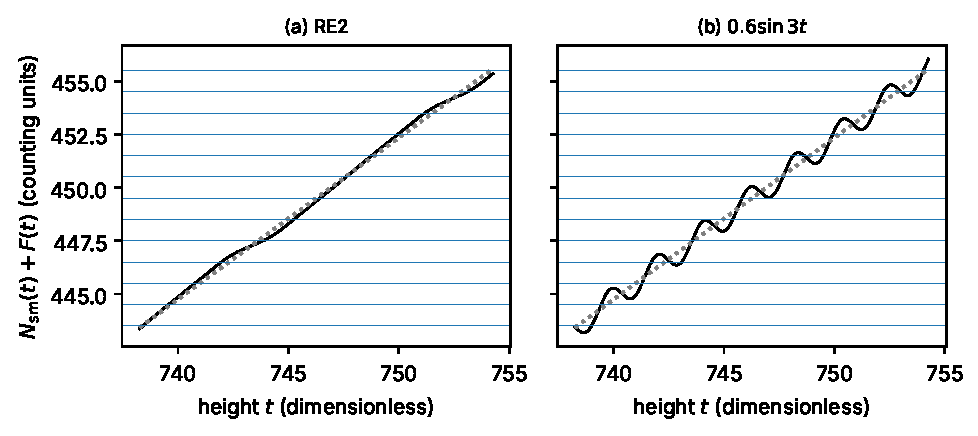
\includegraphics[width=\linewidth]{figs/sparse-frequency_roots.pdf}
\caption{Root ambiguity of the level equation near zero 450 ($t$ dimensionless). Solid: $\Nsm(t)+F(t)$; horizontal lines: the levels $n-\tfrac12$; dotted: $\Nsm(t)$ alone. (a)~$F$ = the prime-2 wave RE2: the curve is increasing, and each level is crossed once. (b)~$F=0.6\sin(3t)$, whose slope reaches $1.8$, above $\Nsm'\approx0.77$: the curve wiggles back, and some levels are crossed three times, so "the" predicted zero is not defined.}
\label{fig:sparse-frequency-roots}
\end{figure}

\subsection{What the paper does about it}

The paper's root finder brackets $\pm3$ mean spacings around $s_n$ and expands the bracket if the sign does not change (Appendix~A step~(8)); Brent's method then returns \emph{one} root in the bracket, which is a choice, not a uniquely defined answer, when several exist. The paper flags its 900-coefficient B row as root-ambiguous: "the level equation has several roots for about a third of the held-out levels", and "the score varies by at most $0.012$ with the choice of root" (Sec.~IV; Table~IV, dagger). Reporting the sensitivity to the arbitrary choice, as the paper does, is the honest response: the row is "not a clean predictive score", but its conclusion (below the null, positively correlated) does not hinge on the choice.

\begin{checkpoint}
If $G_n'(t)>0$ everywhere in a bracket $[a,b]$ and $G_n(a)<0<G_n(b)$, how many roots does $G_n$ have in the bracket?
\end{checkpoint}
\checkanswer{Exactly one. A sign change guarantees at least one crossing, and a strictly increasing function cannot return to zero after crossing it.}

\begin{keyideas}
\item The level equation $\Nsm(t)+F(t)=n-\tfrac12$ has a unique root whenever $\sum_jR_j\omega_j<\Nsm'(t)=\frac1{2\pi}\log\frac{t}{2\pi}$, \eqref{eq:sparse-frequency-monotone}; this is sufficient, not necessary.
\item Large fitted amplitudes, typical of underdetermined fits, can make the model counting function non-monotone and the predicted zero ambiguous.
\item The paper flags such a row and reports how much the score depends on the choice of root.
\end{keyideas}

%======================================================================
\section{Paper connection}\label{sec:sparse-frequency-paper}

This chapter supplies the tools behind one paragraph of methods and one paragraph of results in the paper \cite{soniR1}, together with Table~IV and two steps of its reconstruction record.

\paragraph{Sec.~II~D, "Fitted sinusoidal controls".} The paper explains why it adds these controls: the oracle of Eq.~(4) "is given the functional form", so it is "not a fair ML competitor". All controls have "the shape $\Nsm(t)+F(t)=n-\tfrac12$ with $F(t)=\sum_j[a_j\sin(\omega_jt)+b_j\cos(\omega_jt)]$", are "trained by least squares on $y_n=n-\tfrac12-\Nsm(t_n)$ at the training zeros only", and are "scored exactly as the oracle". These are our \eqref{eq:sparse-frequency-model}, \eqref{eq:sparse-frequency-target} and \eqref{eq:sparse-frequency-level}; \cref{sec:sparse-frequency-why} showed why fitting in $y$ is equivalent, to first order, to fitting the zeros in mean spacings, \eqref{eq:sparse-frequency-errorlink}. Control A is the oracle with up to 300 primes (900 terms, nothing fitted); B fits amplitudes at the given frequencies $m\log p$ (\cref{sec:sparse-frequency-known}); C1 uses 450 frequencies on a uniform grid (\cref{sec:sparse-frequency-dense}); C2 finds $K$ frequencies by greedy periodogram search on $0.05<\omega<8$ with joint refits, $3K$ parameters (\cref{sec:sparse-frequency-greedy}). Ridge strength and $K$ are chosen by the forward 75/25 split of \cref{sec:sparse-frequency-validation}.

\paragraph{Appendix~A step~(20).} This step records the details we used: the ridge filter $\Sigma/(\Sigma^2+\lambda\Sigma_1^2)$, i.e. \eqref{eq:sparse-frequency-ridge}, with $\lambda=10^{-8},\dots,10^3$ in half decades (23 values); the uniform grid $\omega_j=8j/450$; the sparse search with step a quarter of $2\pi/T$, refinement on 201 points, joint refit after each added frequency, and $K\le\min(300,n_{\rm fit}/3)$; scoring as in step~(8) (Brent, bracket $\pm3$ around the smooth zero, expanded on sign failure); and the leakage test (held-out data overwritten with noise, coefficients bit-identical).

\paragraph{Sec.~IV and Table~IV.} The three levels of supplied information are our \cref{tab:sparse-frequency-levels}. Reading the rows of Table~IV with this chapter's tools:
\begin{itemize}
\item A, 300 primes: $0.018$/$+1.00$ on 401--500 and $0.020$/$+1.00$ on 801--1000, interval $[0.015,0.020]$; the oracle "improves monotonically" with budget. Exact frequencies, no dephasing (\cref{sec:sparse-frequency-precision}).
\item B, 25 primes: $0.028$/$+0.99$ and $0.040$/$+0.99$ with 150 fitted amplitudes. B, 150 primes: $0.180$/$+0.78$ and $0.100$/$+0.94$ with 900, underdetermined on 400 zeros (\cref{sec:sparse-frequency-known}) and root-ambiguous (\cref{sec:sparse-frequency-roots}), interval $[0.158,0.201]$.
\item C1: $0.258$/$+0.28$ (interval on the rms $[0.231,0.285]$, on the correlation $[+0.08,+0.46]$) and $0.267$/$+0.22$. Within $0.005$ of the null $0.263$: "capacity without a suitable prior does not generalize, and in this respect the operator family is not special". \Cref{sec:sparse-frequency-dense} derived the kernel form \eqref{eq:sparse-frequency-kernel} and the periodicity \eqref{eq:sparse-frequency-period} that make C1 a generic basis.
\item C2: 24 frequencies (72 parameters) from 400 zeros, $0.034$/$+0.99$, interval $[0.028,0.041]$, "the level of the 25-prime oracle" ($0.043$/$+0.99$); 43 frequencies (129 parameters) from 800 zeros, $0.034$/$+0.99$ on 801--1000.
\end{itemize}
The operator rows ($0.369$/$-0.07$ at $M=400$; $0.313$/$-0.16$ and $0.279$/$-0.03$ at $M=600$; $0.302$/$+0.08$ at $M=900$) come from the paper's Table~I.

\paragraph{The prime-power alignment and Appendix~A step~(23).} The paper reports that "every selected frequency lies within half the Fourier resolution of the training window of the logarithm of a prime power", our criterion \eqref{eq:sparse-frequency-match}, and lists the 43 prime powers we verified in \cref{sec:sparse-frequency-primes}. Because the frequencies are the output of a search, the alignment was rerun on 900 surrogate replicates; the cutoff-maximized binomial score is $24.7$ and $50.9$ on the real zeros and at most $4.7$ on surrogates, with the explicit qualification that the score was "defined after the data were seen". Our density estimate $e^\omega/\omega$ shows why a cutoff matters and why the paper sought a cutoff-free statistic.

\paragraph{Dephasing.} The paper observes that C2's skill "decays with distance from the training window as the estimated frequencies dephase ($0.078$/$+0.96$ on zeros 1001--2000 for the 400-zero fit), which the exact frequencies of the oracle do not". \Cref{sec:sparse-frequency-precision} derived the mechanism, \eqref{eq:sparse-frequency-dephase}--\eqref{eq:sparse-frequency-corr}. The paper's Sec.~VI limits note that "the fitted sinusoidal controls were scored only below zero 2000".

\paragraph{"The obstacle is the parametrization, not the parameter count."} This sentence of the abstract, and the paragraph closing Sec.~IV ("what fails is a potential $V(x)$ as the parametrization"), rest on the combination: C1 (900 coefficients, generic) fails like the potentials; C2 (72 parameters, sparse) succeeds without being told any arithmetic. \Cref{sec:sparse-frequency-prior} spelled out the inductive-bias reading, together with the paper's own hedges: sparsity in frequency is "a strong and well-chosen prior", C2 is "a control built on" the classical Landau--Gonek fact \cite{landau,gonek}, "not a new result", and the explanation of the potentials' failure is heuristic.

\paragraph{Fig.~1 and Table~V.} Fig.~1 of the paper shows the six-prime oracle predicting held-out zeros 401--460 with correlation $+0.96$; Table~V shows the oracle's skill by holdout and prime budget. These are the level-(i) baselines against which C2's level-(ii) result is measured.

%======================================================================
\section{Summary}

\begin{itemize}
\item The training target is one number per zero, $y_n=n-\tfrac12-\Nsm(t_n)\approx S(t_n)$, \eqref{eq:sparse-frequency-target}; it equals minus the fluctuation in mean spacings to high accuracy, \eqref{eq:sparse-frequency-yfluct}, and fitting residuals translate into zero errors by \eqref{eq:sparse-frequency-errorlink}.
\item With frequencies fixed, a sum of sinusoids is linear in its amplitudes, fitted by the normal equations \eqref{eq:sparse-frequency-normal} or the ridge filter \eqref{eq:sparse-frequency-ridge}; amplitude and phase follow from \eqref{eq:sparse-frequency-ampphase}.
\item Columns at frequencies separated by much more than $2\pi/T$ are nearly orthogonal, \eqref{eq:sparse-frequency-orth}: the resolution limit in least-squares form.
\item A uniform frequency grid is exactly periodic, \eqref{eq:sparse-frequency-period}; its ridge fit is a kernel interpolator with the Dirichlet kernel, \eqref{eq:sparse-frequency-kernel}--\eqref{eq:sparse-frequency-dirichlet}. This is why control C1 behaves like a generic basis.
\item A sinusoid of amplitude $A$ gives a periodogram peak $\approx n_{\rm fit}A^2/4$ of width $2\pi/T$, \eqref{eq:sparse-frequency-periodogram}--\eqref{eq:sparse-frequency-peak}; greedy search with joint refits (orthogonal matching pursuit) is control C2.
\item $K$ and the ridge are chosen by a forward split inside the training window; training error alone never selects them.
\item Frequency precision scales as $\sqrt{24}\,\sigma/(A\sqrt n\,T)$, \eqref{eq:sparse-frequency-varomega}; a frequency error dephases as $\phi=\delta\omega\,\Delta t$, \eqref{eq:sparse-frequency-dephase}, giving correlation $\cos\phi$ and rms ratio $2\abs{\sin(\phi/2)}$, \eqref{eq:sparse-frequency-rmsratio}--\eqref{eq:sparse-frequency-corr}.
\item Learned frequencies are matched to prime powers by $\abs{\omega-\log q}<\pi/T$, \eqref{eq:sparse-frequency-match}; amplitudes are $1/(\pi m\sqrt q)$, \eqref{eq:sparse-frequency-amp}; chance matching grows like $e^\omega/\omega$.
\item The level equation has a unique root when $\sum_jR_j\omega_j<\frac1{2\pi}\log\frac t{2\pi}$, \eqref{eq:sparse-frequency-monotone}; large fitted amplitudes can create root ambiguity.
\end{itemize}

%======================================================================
\section{Problems}

\begin{problemlist}
\prob{1}{Control B uses frequencies $m\log p$ with $m=1,2,3$. How many frequencies and how many fitted coefficients does it have with 25 primes? With 150 primes? Which of these two configurations is underdetermined on 400 training zeros?}

\prob{1}{A fitted pair has $a=0.3$, $b=-0.4$. Write $a\sin\omega t+b\cos\omega t$ as $R\sin(\omega t+\varphi)$: find $R$ and $\varphi$.}

\prob{1}{For the 800-zero window take $T=1170$. Compute the resolution $2\pi/T$ and the matching tolerance $\pi/T$. Does a learned frequency $\omega=1.0996$ match $\log3$?}

\prob{1}{A learned component has frequency error $\delta\omega=0.002$. Using \eqref{eq:sparse-frequency-rmsratio}, at what distance from the window centre does its prediction become worse than the null?}

\prob{1}{A ridge grid runs from $10^{-6}$ to $10^{2}$ in half decades. How many values does it contain? Check your method against the paper's grid of 23 values.}

\prob{2}{(a) Prove that $F(t)=\sum_{j=1}^{450}[a_j\sin(j\Delta\omega t)+b_j\cos(j\Delta\omega t)]$ with $\Delta\omega=8/450$ satisfies $F(t+P)=F(t)$ for $P=2\pi/\Delta\omega$. (b) For held-out heights $680<t\le811$, find the two intervals of images $t-P$ and $t-2P$, and say which of them overlap the training window $14\le t\le680$. (c) Exploration: the $p=2$ wave nearly repeats after $P$ (\cref{sec:sparse-frequency-dense}). Compute the phase shift after $P$ of the $p=3$ and $p=5$ waves. Explain why this observation alone cannot tell you whether the periodic images account for C1's small positive correlation, and what computation would.}

\prob{2}{A residual contains two well-separated sinusoids with amplitudes $A_1=0.225$ and $A_2=0.184$, sampled at 400 points over many periods. Estimate the two periodogram peak heights and their ratio. Which is picked first?}

\prob{2}{Derive \eqref{eq:sparse-frequency-corr}: show that the correlation of $\sin\theta$ and $\sin(\theta+\phi)$, averaged over uniformly distributed $\theta$, is $\cos\phi$.}

\prob{2}{Repeat the second matching-pursuit sample with atoms $\bm a=(1,0)$, $\bm b=(0.6,0.8)$ and data $\bm y=0.5\,\bm a+\bm b$. Which atom is picked first? Give the plain matching-pursuit coefficients after two steps, the remaining residual length, and the orthogonal matching-pursuit coefficients.}

\prob{2}{For $F(t)=B\sin(\omega t)$ with $B=0.1$, $\omega=4$, find the height above which \eqref{eq:sparse-frequency-monotone} guarantees a unique root of the level equation.}

\prob{2}{(Paper.) From Table~IV, compute the number of training zeros per fitted parameter for C2 on 400 zeros (72 parameters) and on 800 zeros (129 parameters), and for B with 900 coefficients on 400 and on 800 zeros. Relate the B numbers to the improvement from $0.180$/$+0.78$ to $0.100$/$+0.94$.}

\prob{2}{(Paper.) C1 on zeros 401--500 has rms interval $[0.231,0.285]$ and correlation interval $[+0.08,+0.46]$ (Table~IV caption and Sec.~IV). The null is $0.263$. Does C1 predict better than the null? Is its correlation distinguishable from zero? Explain how both statements can be true at once (recall Chapter~\ref{ch:probability} on rms versus correlation).}

\prob{2}{(Paper, toy model.) Suppose all of C2's held-out error came from the dephasing of a single sinusoid, so that \eqref{eq:sparse-frequency-rmsratio} applies with "null rms" the paper's null. Using C2's $0.034$ on 401--500 (null $0.263$) and $0.078$ on 1001--2000 (null $0.279$, Table~V), find the implied phase errors. Give two reasons the toy model cannot be taken literally.}

\prob{3}{Derive \eqref{eq:sparse-frequency-varomega} in full when both $\omega$ and $\varphi$ are fitted, writing the $2\times2$ normal-equation matrix for $(\delta\omega,\delta\varphi)$ and showing that its off-diagonal entry is small when time is measured from the window centre. What happens to the variance of $\widehat{\delta\omega}$ if time is measured from the start of the window instead and the cross-term is not neglected?}

\prob{2}{(Paper.) Verify that the list "prime powers up to 113 except 32, 64 and 81, and six primes between 131 and 211" contains 43 entries. Which entry corresponds to a term with $m=4$? Compute its amplitude \eqref{eq:sparse-frequency-amp} and compare it with the amplitude of the prime $131$.}

\prob{3}{Using the heuristic density $e^\omega/\omega$ of values $\log p$, find the frequency above which the expected number of $\log p$ values in a matching cell of width $2\pi/T$ exceeds 1, for $T=666$ and for $T=1170$. How do the squares and cubes of primes change the estimate?}

\prob{2}{Using qmnt and numpy, compute $y_n$ for $n\le400$ and its periodogram \eqref{eq:sparse-frequency-periodogram} on the coarse grid of the paper. Where is the largest peak? Does it satisfy \eqref{eq:sparse-frequency-match} for some prime power?}

\prob{2}{Using qmnt and numpy, extend the control-B listing of \cref{sec:sparse-frequency-known}: choose the ridge strength from the paper's 23-value grid by the forward 75/25 split (scoring the validation zeros through the level equation), refit on zeros 1--400, and score zeros 401--500. Compare with the paper's $0.028$/$+0.99$.}

\prob{2}{Using \texttt{qmnt.oracle\_zeros} and \texttt{qmnt.score}, reproduce the six-prime oracle entry of Table~V on zeros 401--500. Then add your result for the sparse model of Problem~20 to a small table alongside it.}

\prob{3}{Using the greedy listing, implement control C2 with $K$ chosen by forward validation (cap $K\le133$), score zeros 401--500 and 1001--2000, and compare with the paper's $0.034$/$+0.99$ and $0.078$/$+0.96$. Report how many of your selected frequencies satisfy \eqref{eq:sparse-frequency-match}.}

\prob{2}{For RE2, the paper's arithmetic-continuation target, find $\max\abs{F'}$ and the threshold height $t^*$ of \eqref{eq:sparse-frequency-monotone}. Can root ambiguity affect the oracle solved with RE2 alone on the paper's holdout 401--500?}

\prob{2}{For the 800-zero window, give the inner fit and validation sizes, the cap on $K$, and the approximate number of coarse search frequencies when $T\approx1170$.}

\prob{3}{Using \eqref{eq:sparse-frequency-varomega}, estimate the precision of the $p=5$ frequency learned from 800 zeros, with $A=0.142$, $\sigma=0.2$, $n=800$, $T=1170$. Express it as a fraction of $\pi/T$. Would you expect weak components such as $q=16$ to satisfy the matching criterion as comfortably?}

\prob{2}{The coarse grid for the 800-zero window has step $\tfrac14\cdot2\pi/T$. Show that the worst-case loss of peak height from the coarse grid alone is the same for every window length, and explain why the refinement step is needed nonetheless.}

\prob{3}{Write a one-page argument, using the first-order level shift $\delta E_n=\int\abs{\psi_n}^2\delta V\,\dd x$ and the localization of sensitivity near turning points (Chapters~\ref{ch:fitting} and~\ref{ch:generalization}), for why a potential fitted to levels 1--400 has no built-in reason to continue a $\sin(t\log 2)$ pattern to levels 401--500. Then state precisely what the paper does and does not claim about this (Secs.~III and~VI).}

\prob{2}{The prime powers $125=5^3$ and $127$ give frequencies $\log125$ and $\log127$. How many resolution cells apart are they for $T=666$? Could the 400-zero window separate them? Which of the two has the larger amplitude?}

\prob{1}{With $T=666$, which of the frequencies $1.3870$, $1.7000$, $2.3979$ satisfy the matching criterion \eqref{eq:sparse-frequency-match}, and with which prime powers?}
\end{problemlist}

%======================================================================
\section{Answers to selected problems}

\textbf{1.} Three frequencies per prime, two coefficients per frequency. 25 primes: 75 frequencies, 150 coefficients. 150 primes: 450 frequencies, 900 coefficients. Only the 900-coefficient model is underdetermined on 400 zeros ($900>400$).

\textbf{2.} $R=\sqrt{0.09+0.16}=0.5$; $\varphi=\operatorname{atan2}(-0.4,0.3)=-0.927$~rad. Check: $0.5\cos(-0.927)=0.3$, $0.5\sin(-0.927)=-0.4$.

\textbf{3.} $2\pi/1170=0.00537$; $\pi/1170=0.002685$. $\abs{1.0996-1.098612}=0.000988<0.002685$: yes, it matches $\log3$.

\textbf{4.} Worse than null when $\phi>\pi/3$, i.e. $\Delta t>(\pi/3)/0.002=524$ (more precisely $523.6$).

\textbf{5.} Exponents $-6,-5.5,\dots,2$: $(2-(-6))/0.5+1=17$ values. The same count for $-8,\dots,3$ gives $11/0.5+1=23$, as in the paper.

\textbf{7.} By \eqref{eq:sparse-frequency-peak} at the peaks, $\mathcal P_1\approx400(0.225)^2/4=5.06$ and $\mathcal P_2\approx400(0.184)^2/4=3.39$, ratio $1.50$. The first ($A_1$) is picked first.

\textbf{9.} $\bm y=(1.1,0.8)$. $\bm y\cdot\bm a=1.1$, $\bm y\cdot\bm b=0.66+0.64=1.3$: $\bm b$ is picked first, coefficient $1.3$. Residual $\bm y-1.3\bm b=(0.32,-0.24)$; $\bm r\cdot\bm a=0.32$, so plain pursuit gives coefficients $0.32$ on $\bm a$ and $1.3$ on $\bm b$, leaving residual $(0,-0.24)$ of length $0.24$. Orthogonal pursuit solves $\alpha+0.6\beta=1.1$, $0.8\beta=0.8$: $\beta=1$, $\alpha=0.5$, residual zero.

\textbf{11.} C2: $400/72=5.56$ and $800/129=6.20$ zeros per parameter. B(900): $400/900=0.444$ and $800/900=0.889$. Both B configurations are underdetermined, but with 800 zeros the data pin down twice as many directions in coefficient space, so the amplitudes are better determined and the held-out score improves.

\textbf{13.} $0.034/0.263=0.129=2\sin(\phi/2)$ gives $\phi\approx0.129$~rad; $0.078/0.279=0.280$ gives $\phi\approx0.280$~rad. Reasons the toy fails: the model has 24 components with different frequency errors and amplitudes, not one; and part of the error is not dephasing at all (omitted terms, amplitude errors, the finite sampling of the window), which is why the error is nonzero even just above the window.

\textbf{15.} $30$ primes up to 113, plus $10$ higher powers ($4,8,16,32,64,9,27,81,25,49$), minus $3$, plus $6$: $43$. The $m=4$ entry is $16=2^4$, amplitude $1/(16\pi)=0.0199$, smaller than the prime 131's $1/(\pi\sqrt{131})=0.0278$; the selection is not a strict ranking by amplitude.

\textbf{17.} The largest peak lies within $\pi/T$ of $\log2=0.6931$ (you should find it within a few thousandths), so it matches the prime power $q=2$. This is the dominant term of RE2, as the amplitude ordering of \cref{tab:sparse-frequency-amps} predicts.

\textbf{19.} You should reproduce Table~V's six-prime entry on 401--500: rms $0.074$ and correlation $+0.96$, the paper's values (Table~V; also Fig.~1). Small differences in the third decimal can come from your bracket or tolerance choices; anything larger points to an error in the prime list or the $m\le3$ truncation.

\textbf{21.} From the RE2 sample, $\max\abs{F'}=\frac{\log2}{\pi}(2^{-1/2}+2^{-1}+2^{-3/2})=0.3443$ and $t^*=2\pi e^{2\pi\times0.3443}\approx54.7$. The holdout 401--500 lies at $t\approx680$--$811$, where $\Nsm'\ge0.745>0.3443$, so by \eqref{eq:sparse-frequency-monotone} every level equation there has exactly one root: no ambiguity.

\textbf{23.} $\sqrt{24}\,(0.2)=0.980$; $0.142\times\sqrt{800}\times1170=4699$; so $\mathrm{std}(\widehat\omega)\approx2.09\times10^{-4}$, which is $0.078$ of $\pi/T=0.002685$. For $q=16$, $A\approx0.020$, the same formula gives about $1.5\times10^{-3}$, roughly $0.55$ of $\pi/T$: a weak component can still match, but much less comfortably, and a match there is closer to a coin toss than for $p=5$.

\textbf{25.} Outline. By first-order perturbation theory, $\delta E_n=\int\abs{\psi_n}^2\delta V\,\dd x$. For high levels, $\abs{\psi_n}^2$ is largest (classically, the particle is slowest) near the turning points $\pm x_{E_n}$, so $\delta E_n$ is dominated by $\delta V$ near $x_{E_n}$. Levels 1--400 have turning points inside a band $\abs x\le x_{E_{400}}$; levels 401--500 turn further out. The training residuals constrain $\delta V$ mainly inside the band; outside it, $\delta V$ is set by whatever the basis functions fitted inside happen to do there, which is fixed by the basis and optimizer, not by a rule that says "continue the oscillation in $t$". Nothing in $\int\abs{\psi_n}^2\delta V$ ties a sinusoid in $E$ (the level heights) to a structure in $x$ that extends itself. The paper claims only what it measured: the probe fit (Sec.~III) represents the $p=2$ wave in-sample (rms $0.056$, corr $+0.95$) and does not continue it (corr $+0.07$); in Sec.~VI it calls the local-versus-global reading heuristic, says the evidence concerns "the tested parametrizations and optimizer together, not a statement about what a potential can represent", and that deriving the memorization result is open.

\textbf{27.} $\pi/T=\pi/666=0.004717$. $\abs{1.3870-\log4}=\abs{1.3870-1.386294}=0.00071$: matches $q=4$. $1.7000$: the nearest prime powers are $5$ ($\log5=1.6094$) and $7$ ($\log7=1.9459$), both far: no match. $\abs{2.3979-\log11}=0.000005$: matches $q=11$.
